
% This must be in the first 5 lines to tell arXiv to use pdfLaTeX, which is strongly recommended.
\pdfoutput=1

\documentclass[letterpaper]{article} % DO NOT CHANGE THIS
\usepackage[submission]{aaai2027}  % DO NOT CHANGE THIS
% The serif, sans-serif, and monospaced fonts are loaded automatically by
% aaai2027.sty (newtxtext, helvet, courier). DO NOT add \usepackage{times},
% \usepackage{helvet}, \usepackage{courier}, or any other font package.
\usepackage[hyphens]{url}  % DO NOT CHANGE THIS
\usepackage{graphicx} % DO NOT CHANGE THIS
\urlstyle{rm} % DO NOT CHANGE THIS
\def\UrlFont{\rm}  % DO NOT CHANGE THIS
\usepackage{natbib}  % DO NOT CHANGE THIS AND DO NOT ADD ANY OPTIONS TO IT
\usepackage{caption} % DO NOT CHANGE THIS AND DO NOT ADD ANY OPTIONS TO IT
\frenchspacing  % DO NOT CHANGE THIS

% Keep the \pdfinfo as shown here. There's no need
% for you to add the /Title and /Author tags.
\pdfinfo{
/TemplateVersion (2027.1)
}

% Number sections and subsections (the maximum AAAI allows) so that
% \Cref{sec:...} and \Cref{app:...} references resolve.
\setcounter{secnumdepth}{2}

\usepackage{latexsym}
\usepackage[utf8]{inputenc}
\usepackage{microtype}
\usepackage{tablefootnote}
\usepackage{amsmath}
\usepackage[capitalize,noabbrev]{cleveref}
\usepackage{xcolor}
\usepackage{amssymb}
\usepackage{makecell}

\newcommand{\Pass}{\textcolor{green}{$\checkmark$}}
\newcommand{\Fail}{\textcolor{red}{$\times$}}
\newcommand{\Todo}{\textcolor{orange}{\textbf{?}}}  % placeholder: axiom result to be supplied

% Voting algorithm names are set in small caps.
\newcommand{\Exact}{\textsc{U-CC-Exact}}
\newcommand{\ExactP}{\textsc{U-CC-Exact}$(\kappa>0)$}
\newcommand{\Greedy}{\textsc{U-CC-Greedy}}
\newcommand{\LP}{\textsc{U-CC-LP}}
\newcommand{\ExactMonroe}{\textsc{U-Monroe-Exact}}
\newcommand{\EExactMonroe}{\textsc{E-Monroe-Exact}}
\newcommand{\Baseline}{\textsc{Baseline}}
\newcommand{\ECCExact}{\textsc{E-CC-Exact}}
\newcommand{\GreedyMonroe}{\textsc{E-Monroe-Greedy}}
\newcommand{\UGreedyMonroe}{\textsc{U-Monroe-Greedy}}

% Fixed-width, left-aligned box so entries in a centered column align on their first character

\title{Chamberlin-Courant Elections with Generative Social Choice}

% Hidden automatically while aaai2027 is loaded with the [submission] option.
\author{
    Aaron Sandoval\textsuperscript{\rm 1},
    Phil Blandfort\textsuperscript{\rm 2}
}
\affiliations{
    \textsuperscript{\rm 1}Independent\\
    \textsuperscript{\rm 2}Predictably Weird\\
    aaron.sandoval10@gmail.com, predictablyweird.com
}

\begin{document}
\maketitle

\begin{abstract}
Large language models (LLMs) present new opportunities for virtual democracy systems to faithfully condense and represent the complex opinions of a constituency.
However, prior systems have limitations such as losing diversity by selecting a single statement, using less expressive ranked ballots, or enforcing excessive constraints that limit the representativeness of outputs.
We build Generative Chamberlin--Courant (GenerativeCC), an LLM-based system that compresses many free-form voter opinions into a small weighted slate of representative statements.
The pipeline (i) summarizes and embeds individual opinions, (ii) generates candidate representative statements, (iii) estimates voter agreement with statements using virtual voters, and (iv) selects a weighted slate using a multiwinner range voting algorithm.
On a dataset of 100 opinions, GenerativeCC outperforms the baseline across all egalitarian and utilitarian social welfare functions.
Ablation studies indicate that the design features primarily driving improved performance are evaluating all voters against all candidate statements, optimizing globally for a utilitarian objective, and allowing the slate to be weighted rather than enforcing equal-sized constituencies.
%While the pipeline runs in exponential time, multiple polynomial time alternatives are presented that achieve similar performance.
GenerativeCC is a practical starting point for virtual democracy systems that represent diverse opinions.
\end{abstract}

\section{Introduction}

\begin{figure}[t]
  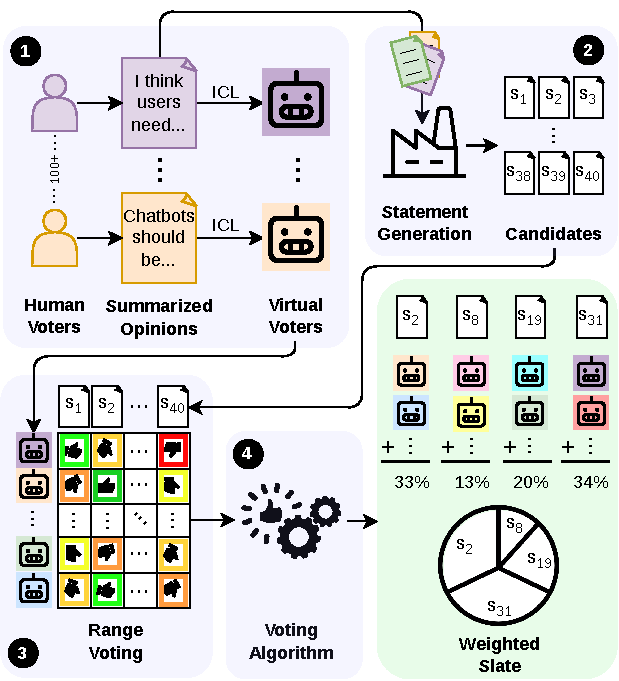
\includegraphics[width=\columnwidth]{figures/Opinion_agg_functionality3.pdf}
  \caption{Overview of GenerativeCC.
  (1) Virtual voters learn to represent individual human opinions using in-context learning (ICL).
  (2) Candidate representative statements are generated from the full population and from clusters of similar voters.
  (3) Virtual voters evaluate candidate statements.
  (4) A voting algorithm selects a weighted slate of representative statements.}
  \label{fig:functionality}
\end{figure}

Recent progress in AI creates both risks and opportunities for collective decision-making \citep{landemore}.
One promising direction is \emph{virtual democracy}, in which multiple AIs representing a constituency help aggregate opinions and support decision-making \citep{noothigattu-2018, kahng-virtual-democracy, freedman-kidney-exchange}.
Recent work has extended this paradigm beyond fixed decision spaces, building voting systems that include large language models (LLMs) to generate and evaluate new candidates in the form of natural language statements \citep{bakker-consensus, habermas-machine, fish-v2, gsc-next-gen}. However, no generative system exists whose  performance has been evaluated on a variety of social welfare functions (SWFs) at a scale of 100+ voters using a realistic dataset of voter opinions.

We design and evaluate such a generative system based on the utilitarian Chamberlin--Courant (CC) rule for multiwinner elections \citep{chamberlin-courant} using range ballots.
We call this system Generative Chamberlin--Courant (GenerativeCC).
The system functionality is illustrated in \Cref{fig:functionality}.
Under the CC rule, a slate of \(k\) winners is selected, where each voter is assigned to their favorite winner as their representative.
Each voter fills out a \emph{range ballot}, scoring every candidate statement by their level of agreement.
A voter's utility is their score for their representative.
For downstream applications, each winner is weighted proportionally to their number of assigned voters.
The CC rule selects the slate and assignment that maximize total utility.
Because each voter counts only their favorite winner, this rule suits our goal of representing diverse views, rather than selecting statements with the broadest appeal \citep{faliszewski-multiwinner-2017, lu-boutilier-2011}.

We use the generative social choice system of \citet{fish-v2} as our baseline.
Relative to their work, GenerativeCC makes two main changes.
First, we allow slate members to represent unequal fractions of the population, rather than enforcing equal constituency sizes as does \citet{monroe-1995}.
Second, we evaluate all voters against all generated candidate statements, yielding a full \emph{ballot profile} and enabling global slate optimization.
These changes allow for separation of statement generation from slate selection and testing of a broader set of voting rules.

We find that GenerativeCC significantly improves over that of \citet{fish-v2} across all tested utilitarian and egalitarian SWFs.
Polynomial-time approximations of the utilitarian CC rule show only slightly worse performance on this dataset.
We perform ablation studies which indicate that the improved performance is primarily due to the two main changes listed above, with other changes having a smaller impact.
GenerativeCC has applications in virtual democracy, automated deliberation systems, or simply as a tool to fairly summarize large collections of free-form opinions.

\paragraph{Our main contributions are:}
\begin{itemize}
    \item We present GenerativeCC, an LLM-based pipeline that combines statement generation, virtual voter utility estimation, and multiwinner range voting.
    On the chatbot personalization dataset of \citet{fish-v2}, we show that this pipeline improves over the closest prior approach across several SWFs.
    \item We evaluate several utilitarian \emph{voting algorithms} against egalitarian baselines on the chatbot personalization dataset and find that (i) the utilitarian algorithms perform better on egalitarian SWFs than baselines that directly optimize minimum utility; (ii) the majority of the improvement in overall pipeline performance is due to the updated voting algorithm; (iii) while axiomatic guarantees are weaker for algorithms that compute a polynomial time approximation, these algorithms perform competitively with an exponential time exact solution on the SWFs.
    This suggests that these approximate solutions could be practical alternatives in terms of solution quality, though testing on more datasets is necessary.
\end{itemize}

\section{Related Work}
\subsection{AI Systems for Virtual Democracy}
GenerativeCC builds directly on that of \citet{fish-v2}.
Their generative social choice system uses virtual voters to both evaluate and generate candidate statements.
We relax from their Monroe election \citep{monroe-1995} with equal-sized constituencies to a CC election \citep{chamberlin-courant} with no such constraint, improve their LLM-based implementation, and use a suite of social welfare functions to measure performance.
In parallel work, \citet{gsc-next-gen} also extends the work of \citet{fish-v2} to build a similar LLM system with theoretical guarantees under more realistic assumptions.
Among their improvements, they apply the same embedding model for clustering statements as GenerativeCC.
\citet{habermas-machine} build a generative virtual democracy system and study its performance with a large scale human study.
While their system uses ranked ballots, selects a single winning statement, and is tested in small groups of up to 6 voters, ours uses more expressive range ballots, selects a weighted slate of winners, and is tested on a single group of 100 opinions.
\citet{polis} describe Polis, a digital democracy system that has been deployed at the scale of thousands of voters to provide a suite of summaries and analyses of voter opinion using iterative voter feedback on each others' statements.
GenerativeCC generates new statements and requires voter input only once, eliminating the bias in Polis related to varying levels and timing of voter participation.
\citet{bakker-consensus} build a generative social choice system using an opinion-conditioned reward model and statement generation model, each fine tuned using data from over 3000 human participants.
GenerativeCC uses more scalable in-context learning \citep{xie-in-context-learning-2021} instead of fine-tuning, and uses a multiwinner rather than a single winner election.

\citet{newberry-moral-parliaments} — and earlier, \citet{bostrom-moral-parliaments-2009} — propose the parliamentary approach to moral uncertainty, an informal decision-making method for individuals which initially inspired this project.
In their approach, various ethical systems with weighted voting power are represented in a simulated parliament, where they bargain and vote on decisions.
GenerativeCC could be applied to select the members in an LLM-based implementation of such a parliament.
\citet{conitzer-2017-moral-ai} envision a similar system using AI, where models of individuals' values vote to make moral decisions.
\citet{noothigattu-2018} and \citet{freedman-kidney-exchange} are the first to apply machine learning and social choice theory to automate ethical decision-making in real applications.
\citet{ouwerx-parliaments} partially implement a simple automated moral parliament, prompting LLM representatives to make compromises to their stances.

\subsection{Voting Systems}
\citet{chamberlin-courant} introduce a system for fully proportional representation in multiwinner elections, where each voter is assigned to one representative, each representative holds a weight proportional to their number of assigned voters, and winners are selected to maximize an objective function.
Our voting algorithms follow this design, but we use range ballots and cardinal utilities instead of their ranked ballots.
The optimal CC slate can be found by solving an integer program \citep{potthoff-brams-1998}, as in our \Exact{} algorithm.
However, this problem is NP-hard \citep{procaccia-2008, lu-boutilier-2011}, so polynomial-time approximations offer a practical alternative. Building the slate greedily, as in our \Greedy{} algorithm, achieves at least $1-1/e$ of the optimal total utility \citep{nemhauser-1978, lu-boutilier-2011}.
Prior works such as \citet{ageev-sviridenko-2004} and \citet{calinescu-2007} find approximate solutions to the CC rule by rounding a linear programming relaxation, using pipage rounding to obtain approximation guarantees.
Our \LP{} algorithm instead selects the $k$ candidates with the largest fractional selection values and assigns each voter to their most preferred selected candidate. This selection method has precedent in participatory budgeting \citep{sreedurga-2022}.

The Kolm--Pollak equally distributed equivalent (EDE) \citep{kolm-1976, pollak-1971} is a social welfare function containing a scalar parameter that interpolates between mean utility and minimum utility. We use it as an objective function, as \citet{horton-2025} do for the problem of facility location.

We do not evaluate other common multiwinner rules such as proportional approval voting, Phragm\'{e}n's sequential method \citep{janson_phragmens_2016}, and the method of equal shares \citep{peters_proportional_2022}, since they consider a voter's satisfaction with all winners rather than only with their assigned representative.

\section{Pipeline}

\subsection{Problem Formulation}
\label{sec:problem-formulation}

We solve the task of compressing a large set of opinions into a small weighted slate of representative statements.
Let \(N=\{1,\ldots,n\}\) be a set of voters, let \(O=(o_1,\ldots,o_n)\) be their free-form opinions on a topic, and let \(k \ll n\) be the desired slate size.
The pipeline generates a set \(A=\{a_1,\ldots,a_m\}\) of \(m \ge k\) candidate statements from \(O\).
As in \citet{fish-v2}, it then selects a slate \(W\subseteq A\) of \(k\) statements together with an assignment \(\omega:N\to W\) mapping each voter to one statement on the slate.
As in the Chamberlin--Courant rule \citep{chamberlin-courant, skowron-2015}, each statement \(a\in W\) is weighted by the fraction of voters assigned to it, \(|\omega^{-1}(a)|/n\), where \(\omega^{-1}(a)=\{i\in N:\omega(i)=a\}\).

\paragraph{Objective}
Following \citet{chamberlin-courant,fish-v2}, we model voter utility as their level of agreement with their assigned statement.
GenerativeCC seeks to maximize total voter utility, or related quantities.

\subsection{Algorithm}

\begin{enumerate}
    \item Use voter opinions \(O\) to generate the candidate statements \(A\).
    \begin{enumerate}
        \item For each opinion \(o_i\), generate a summary of roughly standard length.
        In our case study, we reuse the summaries from \citet{fish-v2}, each under 50 words.
        \item Embed each summary %We use OpenAI's \texttt{text-embedding-3-small}.
        and perform k-means on the embedding vectors to cluster opinions.
        \item Generate candidate statements from the full population and from individual clusters.
        In our experiments, GPT-4o performs all candidate-generation requests.
        See \Cref{sec:statement-generation} for details.
    \end{enumerate}

    \item Compute the ballot profile \(U\in \mathbb{R}^{n\times m}\) over voters \(N\) and candidate statements \(A\).\footnote{The method for computing \(U\) is nearly identical to that of \citet{fish-v2}.
    The main differences are that we compute utilities only after all statements are generated, we compute the full matrix \(U\), and we use a different LLM.}
    \begin{enumerate}
        \item Model each voter's utility function with a virtual voter, implemented using in-context learning \citep{xie-in-context-learning-2021} with GPT-4o mini.
        The prompt includes \(o_i\) and ends with candidate statement \(a_j\), requesting a 0--4 Likert score.
        \item For each pair \((i,j)\), compute the expected Likert score \(U_{ij}\) assigned by the virtual voter \(i\) to the candidate \(a_j\) by taking the average weighted by token-probability over the responses 0--4.
        We treat this expected score as voter \(i\)'s agreement with \(a_j\).
        \item Repeat steps (a) and (b) for all \(i\in N\) and \(j\in[m]\).
    \end{enumerate}

    \item Apply a voting algorithm to \(U\) to select a winning slate \(W\subseteq A\) of size \(k\) and an assignment \(\omega:N\to W\).
    \begin{enumerate}
        \item Unless otherwise noted, we select the slate that maximizes total utility using an exact integer-programming formulation solved with PuLP/CBC \citep{pulp, john_forrest_cbc}.
        We compare several alternative voting rules in \Cref{sec:voting-algorithms}.
    \end{enumerate}
\end{enumerate}

\subsection{Statement Generation Details}
\label{sec:statement-generation}

We generate candidates in three stages: (i) compute embeddings for all voters, (ii) cluster voters, and (iii) generate statements for the whole population and for individual clusters.

For embeddings, we consider two notions of similarity.

\paragraph{LLM embeddings}
We embed each opinion summary with OpenAI's \texttt{text-embedding-3-small} and measure cosine similarity.

\paragraph{Discriminative distances \citep{fish-v2}}
We ask voter \(j\) to rate the summary statement of voter \(i\).

In GenerativeCC, we cluster voters with \(k\)-means on the LLM embeddings, using five clusters.

Given a set of opinions, we then generate candidates in two ways.

\paragraph{Single-statement generator}
Generate one statement intended to represent the set of opinions; we run this generator twice.

\paragraph{Batch generator}
Generate five statements at once, prompted to jointly represent the set of opinions as well as possible.

We apply both generators once to the set of all opinions and once to each of the five clusters.
This yields
\[
\begin{aligned}
&(2\,\text{from single\text{-}statement generator} \\
&\quad + 5\,\text{from batch generator}) \\
&\times (1\,\text{population} + 5\,\text{clusters}) \\
&= 42\,\text{candidate statements}
\end{aligned}
\]
In our experiments, we use GPT-4o with temperature 1 for all generative queries.
Across runs, all statement generation methods contribute statements that are eventually selected into a final slate.
\Cref{app:statement-origin} reports the breakdown by generator.

\subsection{Inference Costs and Runtime Complexity}

\paragraph{Inference costs}
For a fixed number of generated candidates, GenerativeCC uses roughly twice as many LLM calls as that of \citet{fish-v2} (see \Cref{tab:llm-call-comparison}).

\paragraph{Runtime complexity}
In practice, runtime is dominated by LLM calls, which are comparable in cost per call across the baseline and GenerativeCC.
Beyond LLM inference, GenerativeCC performs \(k\)-means clustering on embeddings and then runs one of the voting algorithms from \Cref{sec:voting-algorithms}, which may have polynomial or exponential runtime (\Cref{tab:time-complexity}).
However, at the small scale of our experiments, GenerativeCC is slower mostly due to the linear difference in required LLM inference rather than any difference in voting algorithm runtime.

\paragraph{Number of generated statements}
For both approaches, the number \(m\) of generated candidates is a multiple of the number of statement-generation methods used.
If \(g\) denotes the number of generators, the baseline produces \(m=k\cdot g\) candidates, while GenerativeCC produces \(m=(c+1)\cdot g\), where \(c\) is the number of clusters.

\begin{table*}[t]
\centering
\begin{tabular}{lcc}
\hline
Type of LLM Call & GenerativeCC & Baseline \citep{fish-v2} \\
\hline
Get opinion embedding & $n$ & -- \\
Generate a candidate & $m$ & $m$ \\
Rate a candidate & $nm$ & $\frac{1}{2} n m (1 + 1/k)$ \\
\hline
\end{tabular}
\caption{Number of calls for different types of LLM requests for running the full pipeline, where \(m\) is the number of generated candidates, \(n\) the number of voters, and \(k\) the slate size.
The baseline requires \(m\) to be a multiple of the slate size, while GenerativeCC allows \(m\) to be chosen more freely so long as \(m\ge k\).}
\label{tab:llm-call-comparison}
\end{table*}

\section{Experimental Setup}

We evaluate our full pipeline on the chatbot personalization survey of \citet{fish-v2}.
Throughout, we compare against results obtained by running their pipeline under matched model choices.

\subsection{Input Data}

The chatbot personalization dataset contains survey responses from a representative sample of 100 U.S.\ residents.
In addition to free-form responses, the survey asks participants to rate one of seven seed statements about chatbot personalization on a 0--4 Likert scale.
For details, see Section 5 of \citet{fish-v2}.

Rather than using the original survey responses directly, we use the summarized participant responses released by \citet{fish-v2}.\footnote{The original data are available at \url{https://github.com/generative-social-choice/chatbot_personalization}.}

\subsection{Baseline}

We run the pipeline of \citet{fish-v2} with two modifications for a cleaner comparison:
\begin{enumerate}
    \item We start from their released summaries rather than re-running the summarization step.
    \item We use GPT-4o for generative queries and GPT-4o mini for discriminative queries, matching the model choices in our own pipeline.
\end{enumerate}

\subsection{Evaluation Metrics}
\label{sec:metrics}

For each run, we compute the social welfare functions of average utility, average utility among the bottom 50\% of voters, minimum utility, the Gini coefficient \citep{gini}, and mean log utility.
The latter is proportional to the Nash welfare function \citep{nash-welfare}.
Voter utility is assumed equal to the Likert score returned by the virtual voter's discriminative query for their assigned statement.

We produce multiple samples using each method and use bootstrapping to estimate confidence intervals of mean performance.
The number of runs differs across methods and is reported in the result figures.

\section{Case Study Results}

\paragraph{Overall performance}
Across the scalar metrics we consider, GenerativeCC outperforms the baseline of \citet{fish-v2} (\Cref{fig:swf-main}).
Both distributions are similar in the top half, but a difference grows in the lower tail (\Cref{fig:mth-happiest-main}), indicating superior performance by both egalitarian and utilitarian standards.

\begin{figure*}[t]
  \begin{center}
  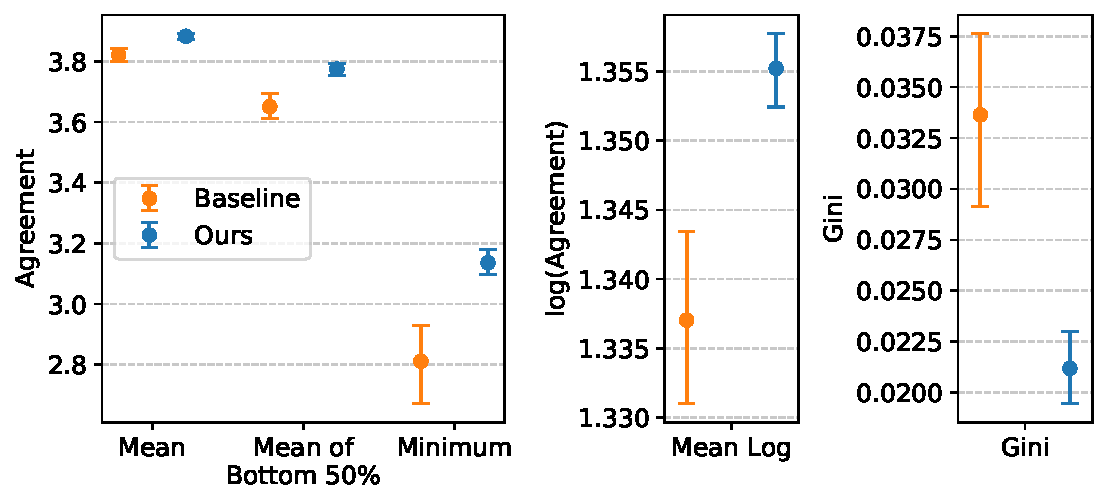
\includegraphics[width=0.6\textwidth]{figures/scalar_confidence_intervals.pdf}
  \caption{GenerativeCC outperforms the most closely related approach from \citet{fish-v2} on five utilitarian and egalitarian social welfare functions.}
  \label{fig:swf-main}
  \end{center}
\end{figure*}

\begin{figure*}[t]
  \begin{center}
  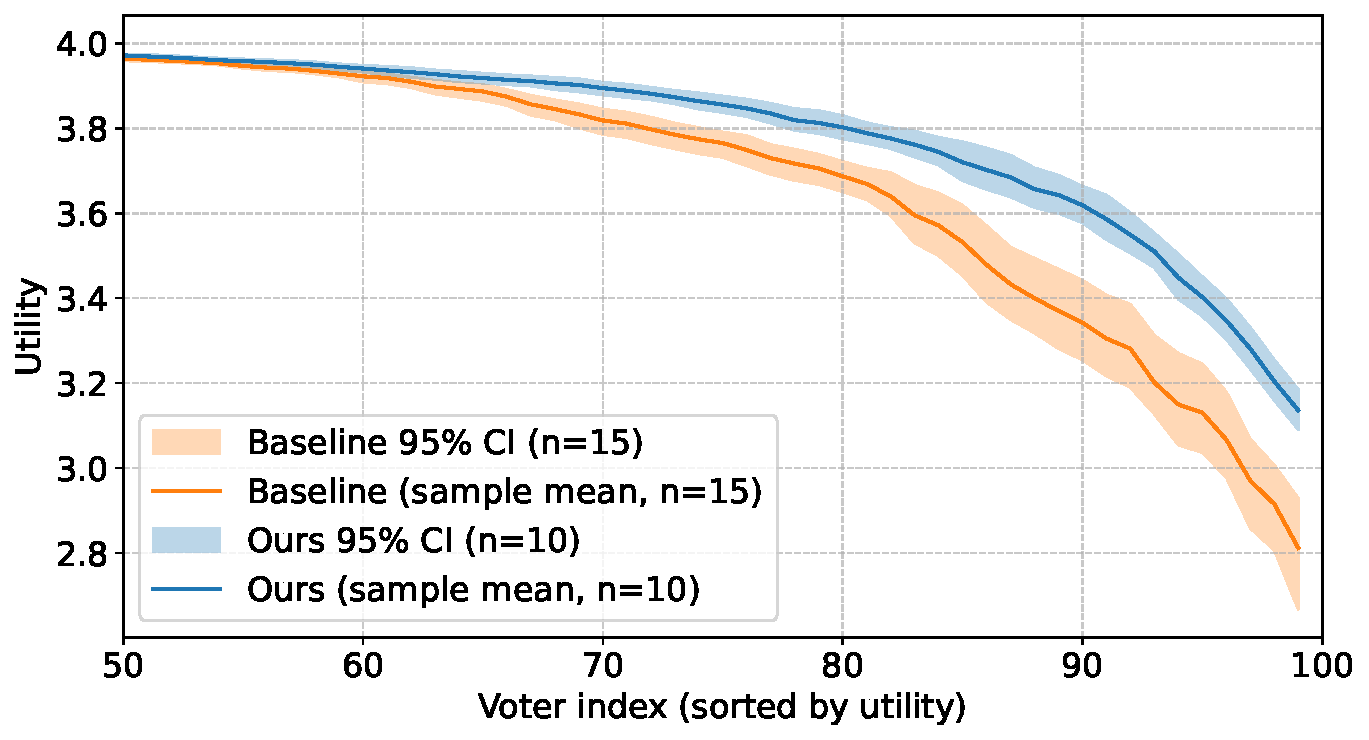
\includegraphics[width=0.7\textwidth]{figures/sorted_utility_CIs_main.pdf}
  \caption{Confidence intervals for the mean sorted vector of voter utilities on the chatbot personalization dataset.
  Only the bottom 50\% of voters are shown; the upper 50\% are visually indistinguishable at this scale.}
  \label{fig:mth-happiest-main}
  \end{center}
\end{figure*}

\paragraph{Ablation studies}
To investigate the mechanisms behind the performance gap, we separately ablate our embeddings and the larger number of candidates generated by GenerativeCC.
We find that these each account for a relatively small performance difference.

First, we run a statement count ablation.
GenerativeCC generates 42 candidates while the baseline generates 30.
In that ablated variant, we subsample the 5 statements output from the batch generator, retaining 3 at random.
Since this generator is applied once to the full population and once to each of five clusters, the total number of candidates drops from 42 to 30, matching the baseline.
As detailed in~\Cref{app:statement-ablation-details}, this has little effect on performance.
The gap to the baseline remains nearly unchanged, suggesting that our gains are not driven primarily by a larger candidate pool.

Second, we ran an embedding ablation in both directions: we both substitute our LLM embeddings into the baseline pipeline and also substituted the baseline's embeddings into GenerativeCC.
As shown in \Cref{app:embedding-ablation-details}, these changes have only limited effects on either method.
This suggests that better clustering is also not the main explanation for the performance gap.

We do not run any study varying model selection, but we believe model selection unlikely to be a major contributor to the performance difference.
While \citet{fish-v2} uses three variants of GPT-4, all of our experiments, including those on their pipeline, use GPT-4o mini and GPT-4o.
It's possible that this could account for a small difference, but only if either pipeline were overfit to the particular models used to test them.

Removing the above factors, we conclude that the changes in the voting process and voting algorithm account for most of the improvement.
More specifically, these changes are (i) computing the complete ballot profile $U$ and using voting algorithms that act on the full profile at once; (ii) using a utilitarian voting algorithm rather than an approximated egalitarian variant of the Greedy Monroe rule \citep{skowron-2015}; (iii) lifting the constraint of approximately equal numbers of voters assigned to each winning statement.

\section{Voting Algorithms}
\label{sec:voting-algorithms}

We compare voting algorithms independently of the rest of the pipeline.
In GenerativeCC, a voting algorithm selects candidates in a multiwinner election and maps each voter to exactly one winner.
We implement voting algorithms for range ballots and evaluate them against a set of social choice axioms and the social welfare functions in \Cref{sec:metrics}.

\subsection{Algorithms}
\label{sec:algorithms}

We evaluate \textsc{CC} algorithms as candidates for GenerativeCC, and \textsc{Monroe} algorithms as ablations relative to the baseline of \citet{fish-v2}.
Most of these algorithms sit in a three-dimensional design space, parametrized by the objective function, the constituency-size constraint, and the solution method (\Cref{tab:algorithm-space}).
Their names list their coordinates in this order, e.g.\ \Exact{} maximizes total utility exactly under the CC rule.
The remaining algorithms do not fit this space and are described afterwards.

\begin{table*}[t]
\centering
\begin{tabular}{ll|ccc}
\hline
\textit{Rule} & \textit{Method} & Utilitarian & Kolm--Pollak & Egalitarian \\
\hline
CC & Exact & \Exact{} & \ExactP{} & \ECCExact{} \\
 & Greedy & \Greedy{} & -- & -- \\
 & LP & \LP{} & -- & -- \\
\hline
Monroe & Exact & \ExactMonroe{} & -- & \EExactMonroe{} \\
 & Greedy & \UGreedyMonroe{} & -- & \GreedyMonroe{} \\[3pt]
 & \makecell[l]{Interleaved\\Greedy} & -- & -- & \Baseline{} \\[2pt]
\hline
\end{tabular}
\caption{Specification and names of most of the tested voting algorithms within a 3-dimensional design space: constituency-size constraint (rule), solution method (method), and objective function (columns). We show results for the named entries.}
\label{tab:algorithm-space}
\end{table*}

\paragraph{Objective function}
Utilitarian (U-) algorithms maximize the total utility \(\sum_i U_{i,\omega(i)}\) of the assignment.
Egalitarian (E-) algorithms maximize the minimum utility \(\min_i U_{i,\omega(i)}\).
Between these, \ExactP{} maximizes the Kolm--Pollak equally distributed equivalent (EDE) \citep{kolm-1976, pollak-1971} instead of total utility.
For an inequality aversion parameter \(\kappa>0\), the EDE of utilities \(u_1,\dots,u_n\) is
\[
\mathrm{EDE}_\kappa(u)=-\frac{1}{\kappa}\ln\Bigl(\frac{1}{n}\sum_{i=1}^n e^{-\kappa u_i}\Bigr).
\]
\ExactP{} replaces each utility \(U_{ij}\) in the ballot profile with \(f(U_{ij})\), where
\[
f(u)=\frac{1-e^{-\kappa u}}{1-e^{-\kappa}},
\]
and then runs \Exact{} on the transformed ballot profile.\footnote{For numerical stability the solver uses equivalent utilities \(-e^{\kappa(c-U_{ij})}\), where \(c=\min_i\max_j U_{ij}\); this is a positive affine transformation of \(f\) and selects the same slate and assignment, but avoids the near-constant values of \(f\) at large \(\kappa\).}
The total transformed utility \(\sum_i f(U_{i,\omega(i)})\) is a strictly increasing function of the Kolm--Pollak EDE of the original utilities, so the two objectives select the same slate and assignment.
The parameter \(\kappa\) interpolates between utilitarian social welfare (total utility) as \(\kappa\to0\) and egalitarian social welfare (minimum utility) as \(\kappa\to\infty\).

\paragraph{Constituency size constraint}
Under the CC rule \citep{chamberlin-courant}, each voter is assigned to their favorite winner, and constituencies may have any size.
The Monroe rule \citep{monroe-1995} instead assigns each winner an equal-sized constituency of either \(\lfloor n/k\rfloor\) or \(\lceil n/k\rceil\) voters, as in the pipeline of \citet{fish-v2}.

\paragraph{Solution method}
\textsc{Exact} algorithms select the slate and assignment that optimize the objective exactly, by solving an integer program (\Cref{app:exact-lp-formulations}).
\textsc{Greedy} algorithms build the slate one candidate at a time in \(k\) rounds.
\textsc{Greedy} algorithms proceed differently depending on the constituency size constraint.
In \textsc{CC-Greedy} algorithms, each round selects the candidate that scores highest on the objective function and assigns every voter to their favorite slate member.
We do not define \textsc{E-CC-Greedy}: a new winner raises the minimum utility only if it improves every voter at the minimum, so in most rounds all remaining candidates tie on the egalitarian objective and the selection is left to tie-breaking.
\textsc{Monroe-Greedy} algorithms instead score each remaining candidate only over the voters not yet assigned.
In each round, a candidate's objective function is computed only over the \(\lceil n/k\rceil\) unassigned voters with the highest utility for it.\footnote{(\(\lfloor n/k\rfloor\) in the last rounds if \(k \nmid n\))}
Upon selecting a winner, those voters are permanently assigned to that winner.

\LP{} approximates \Exact{} with a linear program: it uses the same problem formulation for slate selection and voter assignment as \Exact{}, %assignment-and-selection formulation as Exact,
but relaxes binary constraints to the interval \([0,1]\).
After solving the relaxed program, it selects the \(k\) candidates with largest fractional values and assigns each voter to their most preferred selected candidate.

\paragraph{\Baseline{} \citep{fish-v2}}
The baseline pipeline selects its slate with the same rule as \GreedyMonroe{}, but interleaves selection with statement generation.
In each of the \(k\) rounds, \(m/k\) new candidates are generated from the opinions of the unassigned voters, and only the unassigned voters rate them.
The candidates generated in earlier rounds that are not yet on the slate remain eligible.
One candidate is selected, its voters assigned, and the roudn concludes.
This uses \(\frac{1}{2} n m (1 + 1/k)\) discriminative queries instead of \(nm\) (\Cref{tab:llm-call-comparison}).

\paragraph{\Baseline{} + \EExactMonroe{} reassign}
In some use cases, discriminative queries may be expensive, and it may be desirable to incur a performance cost to avoid computing a full ballot profile.
Still, better SWF performance than that of the baseline can be attained with relatively few additional queries.
This algorithm selects the slate using \Baseline.
Then, full discriminative queries are performed on the slate.
Finally, voters are reassigned with \EExactMonroe{}.
This algorithm uses at most \(\frac{1}{2} n (m + m/k + k - 1)\) total discriminative queries, compared with \(nm\) for the algorithms that compute the full ballot profile and \(\frac{1}{2} n (m + m/k)\) for the baseline (\Cref{tab:llm-call-comparison}).

\paragraph{\Baseline{} + CC reassign}
Similar to \Baseline{} + \EExactMonroe{} reassign, but the Monroe constraint is removed and each voter is assigned to their favorite member of the slate.

\subsection{Axioms}
\label{sec:axioms}

In addition to the social welfare metrics used in the case study, we evaluate the \textsc{U-CC} voting algorithms against a set of social choice axioms.
The axioms are criteria expressed in terms of the algorithm's selected voter assignment $\omega$, and some alternative voter assignment $\omega'$ that was not selected.
To satisfy an axiom, the criteria must hold for all possible ballot profiles $U$ and all possible $\omega'$ for each profile, except for cases where the utilities for multiple slates or candidates have identical sums.
Since the discriminative query returns floating-point-valued utilities, and all of the voting algorithms under study are additive, such collisions are exceedingly rare in practice.
We consider an axiom to have failed only if a counterexample ballot profile that does not contain such a collision can be specified.
Write $u_\omega=(U_{1,\omega(1)},\ldots,U_{n,\omega(n)})$ for the utility vector realized by an assignment $\omega$, and let $u_{\omega,(1)}\le\cdots\le u_{\omega,(n)}$ denote its ascending sort.

\paragraph{Symmetry}
Changing the order of voters or statements in the ballot profile $U$ does not change $\omega$.

\paragraph{Independence of Common Scale}
Linearly scaling all utilities by a positive constant never changes $\omega$.

\paragraph{Monotonicity}
Increasing (decreasing) a voter’s rating for a winning (losing) candidate never causes that candidate to lose (win).

\paragraph{Individual Pareto Efficiency}
No $\omega'$ \emph{Pareto-dominates} $\omega$, meaning no $\omega'$ increases total utility without decreasing any individual voter's utility.
Formally, $U_{i,\omega'(i)}\ge U_{i,\omega(i)}$ for all $i$ with at least one strict inequality.

\paragraph{Sorted Pareto Efficiency \citep{sorted-pareto}}
No $\omega'$ \emph{sorted-Pareto-dominates} $\omega$, meaning no $\omega'$ has a sorted utility vector that Pareto-dominates that of $\omega$.
Formally, $u_{\omega',(\ell)}\ge u_{\omega,(\ell)}$ for all $\ell$ with at least one strict inequality.
Sorted Pareto Efficiency implies Individual Pareto Efficiency (see \Cref{app:axiom-implications} for proof).

\paragraph{Generalized Lorenz Efficiency \citep{shorrocks-1983}}
No $\omega'$ \emph{generalized-Lorenz-dominates} $\omega$, meaning no $\omega'$ has a generalized Lorenz curve that dominates that of $\omega$.
Formally, $\sum_{\ell=1}^{j}u_{\omega',(\ell)}\ge\sum_{\ell=1}^{j}u_{\omega,(\ell)}$ for all $j$ with at least one strict inequality.
Equivalently, when all voters are anonymized, it is impossible to select an $\omega'$ such that the anonymous transformation of $u_{\omega}$ to $u_{\omega'}$ can be expressed as a non-empty series of actions either granting positive utility to a voter or transferring utility from "wealthier" voters to "poorer" voters without reversing their order \citep[Thm.~1]{kostreva-ogryczak-wierzbicki-2004}.
Generalized Lorenz Efficiency implies Sorted Pareto Efficiency (see \Cref{app:axiom-implications} for proof).

\paragraph{Egalitarian--Utilitarian Efficiency}
No $\omega'$ has both greater total and minimum utility.

\paragraph{Non-radical Utilitarianism}
No $\omega'$ has marginally lower total utility and substantially higher minimum utility.
More formally, with the selected slate $\omega$ having total utility $u_{\mathrm{tot}}$ and minimum utility $u_{\mathrm{min}}$ there exists no $\omega'$ with total utility $u_{tot} - \delta$ and minimum utility $u_{\mathrm{min}} + \epsilon$, where $\epsilon > 0, \delta > 0$ and $\epsilon/\delta$ is arbitrarily large.

We do not aim to satisfy committee monotonicity \citep{elkind-committee-monotonicity} or balanced justified representation \citep{fish-v2}.
\Cref{tab:committee-monotonicity-example,tab:bjr-example} illustrate why these properties may be undesirable for representative slate generation.

\begin{table}[t]
\centering
\begin{tabular}{l|ccc}
\hline
 & $a_1$ & $a_2$ & $a_3$ \\
\hline
Voter 1 & 2 & 3 & 0 \\
Voter 2 & 2 & 0 & 3 \\
\hline
\end{tabular}
\caption{Example ballot profile where violating committee monotonicity is desirable when increasing the slate size from \(k=1\) to \(k=2\).}
\label{tab:committee-monotonicity-example}
\end{table}

\begin{table}[t]
\centering
\begin{tabular}{l|cc}
\hline
 & $a_1$ & $a_2$ \\
\hline
Voter 1 & 1 & 0 \\
Voter 2 & 1 & 0 \\
Voter 3 & 1 & 0 \\
Voter 4 & 0 & 1 \\
\hline
\end{tabular}
\caption{Example ballot profile with \(k=2\) where enforcing BJR reduces utility for one of voters 1, 2, and 3.
Under BJR, \(a_1\) and \(a_2\) must have equal numbers of voters assigned.}
\label{tab:bjr-example}
\end{table}

\subsection{Results}
\label{sec:voting-results}

We evaluate voting rules against each axiom using a set of adversarial ballot profiles.
These profiles are generated both manually and using LLMs (ChatGPT 5.3 and Claude Opus 4.7).
For \Exact{}, we provide formal proofs of satisfaction of some axioms in \Cref{app:exact-axiom-proofs}.
As we don't provide formal proofs of satisfaction for other voting algorithms, false positives remain possible, but any hypothetical false positives wouldn't affect our conclusions.
Results are shown in \Cref{tab:voting-axioms}. %These are best-effort empirical checks rather than formal proofs of satisfaction, so false positives remain possible.
Counterexamples for key axiom failures are provided in \Cref{app:voting-failures}.

\begin{table*}[t]
\centering
\small
\setlength{\tabcolsep}{4pt}
\begin{tabular}{lcccc}
\hline
 & \Exact{} & \ExactP{} & \Greedy{} & \LP{} \\
\hline
Independence of Common Scale
& \Pass
& \Fail\tablefootnote{The Kolm--Pollak EDE is invariant to a common additive shift of utilities rather than to a common scaling \citep{blackorby-donaldson-1980}; see \Cref{app:exactp-ics}.}
& \Pass
& \Pass \\

Symmetry
& \Pass
& \Pass
& \Pass
& \Fail\tablefootnote{See \Cref{app:lp-worst}.} \\

Monotonicity
& \Pass
& \Pass
& \Pass
& \Fail\tablefootnote{See \Cref{tab:lp-monotonicity}.} \\

Individual Pareto Efficiency
& \Pass
& \Pass
& \Fail\tablefootnote{Shown by \citet{lackner-skowron-2020} Example 4 for approval ballots, a special case of range ballots for which \Greedy{} is equivalent to sequential Chamberlin--Courant. See also \Cref{tab:failure-greedy-indiv-pareto}.}
& \Fail\tablefootnote{See \Cref{tab:lp-fractional}.} \\

Sorted Pareto Efficiency
& \Pass
& \Pass
& \Fail
& \Fail \\

Generalized Lorenz Efficiency
& \Pass\tablefootnote{Satisfaction depends on the no-ties condition of \Cref{sec:axioms} \citep{kostreva-ogryczak-wierzbicki-2004}.}
& \Pass\tablefootnote{Shown by \citet[Cor.~2]{kostreva-ogryczak-wierzbicki-2004} for any strictly concave, increasing utility transformation.}
& \Fail
& \Fail \\

Egalitarian--Utilitarian Efficiency
& \Pass
& \Fail\tablefootnote{\Cref{tab:egal-util-strict} is a counterexample at \(\kappa=\ln 1.5\).}
& \Fail
& \Fail\tablefootnote{See \Cref{tab:lp-fractional}.} \\

Non-radical Utilitarianism
& \Fail\tablefootnote{See \Cref{app:exact-nru}.}
& \Fail\tablefootnote{See \Cref{app:exactp-nru}.} %\Pass\tablefootnote{This passes only when utilities are bounded, as in our experiments, and \(p\) is only infinitesimally greater than 1.}
& \Fail
& \Fail \\
\hline
\end{tabular}
\caption{Performance of \textsc{CC} voting algorithms against social choice axioms.}
\label{tab:voting-axioms}
\end{table*}

\begin{table}[t]
\centering
\footnotesize
\setlength{\tabcolsep}{4pt}
\begin{tabular}{lccc}
\hline
 & \multicolumn{3}{c}{Worst-case time} \\
Algorithm & Exp. & Poly. & Indep. \\
\hline
\Exact{} & \(n,m\)\tablefootnote{Solver-dependent: the implementation solves integer programs by branch-and-bound (\Cref{app:brute-force-vs-exact}); \ECCExact{} solves a sequence of polynomially many in \(n\) (\Cref{app:exact-lp-formulations}).
Enumerating all \(\binom{m}{k}\le 2^m\) slates instead and computing each slate's assignment directly is exponential only in \(m\), and polynomial in \(n\) and \(k\).}\xdef\exactcomplexityfn{\number\value{footnote}} & -- & \(k\) \\ \hline
\Greedy{} & -- & \(n,m,k\) & -- \\ \hline
\LP{} & \(n,m\)\tablefootnote{Solver-dependent.
The simplex method we use has an exponential worst case; an interior-point method makes \LP{} polynomial in \(n\) and \(m\).
See \Cref{app:lp-complexity}.} & -- & \(k\) \\ \hline
\ExactMonroe{} & \(n,m\)\tablefootnote{Solver-dependent: the implementation solves integer programs by branch-and-bound (\Cref{app:brute-force-vs-exact}); \EExactMonroe{} solves a sequence of polynomially many in \(n\) (\Cref{app:exact-lp-formulations}).
Enumerating all \(\binom{m}{k}\le 2^m\) slates instead and computing each slate's assignment as a flow problem is exponential only in \(m\), and polynomial in \(n\) and \(k\) (\citealp[Prop.~2]{betzler-2013}; \Cref{app:baseline-reassign-complexity}).}\xdef\monroecomplexityfn{\number\value{footnote}} & -- & \(k\) \\ \hline
\ExactP{} & \(n,m\)\footnotemark[\exactcomplexityfn] & -- & \(k\) \\ \hline
\ECCExact{} & \(n,m\)\footnotemark[\exactcomplexityfn] & -- & \(k\) \\ \hline
\EExactMonroe{} & \(n,m\)\footnotemark[\monroecomplexityfn] & -- & \(k\) \\ \hline
\UGreedyMonroe{} & -- & \(n,m,k\) & -- \\ \hline
\GreedyMonroe{} & -- & \(n,m,k\) & -- \\ \hline
\makecell[l]{\Baseline{} +\\\EExactMonroe{} reassign} & \(n,k\)\tablefootnote{Solver-dependent: the reassignment solves integer programs by branch-and-bound over the baseline's slate only, and \(m\) enters only through the baseline's slate selection.
With the slate fixed, the reassignment can instead be computed as a minimum-cost flow, which is polynomial in \(n\), \(m\), and \(k\); see \Cref{app:baseline-reassign-complexity}.} & \(m\) & -- \\ \hline
\makecell[l]{\Baseline{} +\\CC reassign} & -- & \(n,m,k\) & -- \\
\hline
\end{tabular}
\caption{Worst-case time complexity of the voting algorithms as implemented, where \(k\) is the slate size, \(m\) the number of candidates, and \(n\) the number of voters.
Each row represents a complexity of \(O(2^{f}\cdot g)\), where \(f\) is a polynomial in the variables in the \textit{Exp.}\ (exponential) column, \(g\) is a polynomial in the variables in the \textit{Exp.}\ and \textit{Poly.}\ (polynomial) columns, and neither depends on the variables in the \textit{Indep.}\ (independent) column.
These are upper bounds for our implementations (see \Cref{app:brute-force-vs-exact}), not for the underlying problems.}
\label{tab:time-complexity}
\end{table}

\begin{figure*}[t]
\centering
  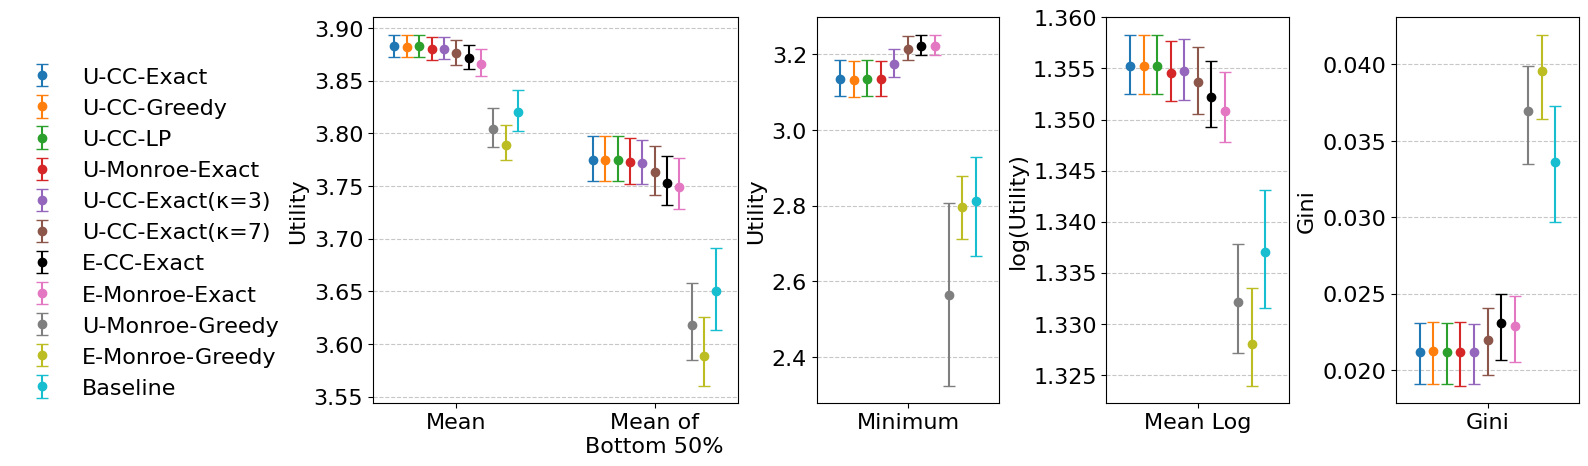
\includegraphics[width=\textwidth]{figures/voting_alg_scalar_metrics_v8.png}
  \caption{Mean voting algorithm performance on social welfare functions for a slate size of 5.
  Confidence intervals for all series except \Baseline{} are bootstrapped across 10 ballot profiles generated with GenerativeCC.
  The \Baseline{} series is copied from \Cref{fig:swf-main}. It was generated from the pipeline of \citet{fish-v2} and is included for reference only.
  Its results are not directly comparable as other pipeline elements besides the voting algorithm differ.}
  \label{fig:sfws-voting-algs}
\end{figure*}

We also evaluate each voting algorithm on the social welfare functions from \Cref{sec:metrics}.
Using the 10 ballot profiles generated from GenerativeCC with LLM embeddings in the embedding ablation study (Appendix~\ref{app:embedding-ablation-details}), we produce the results in Figure~\ref{fig:sfws-voting-algs}.
We show \ExactP{} with stronger inequality aversion \(\kappa=3\) and \(\kappa=7\) because a mild transformation behaves almost identically to \Exact{} on this dataset.
All differences quoted below are in utility on the 0--4 Likert scale, averaged over profiles.
Since every voting algorithm in \Cref{fig:sfws-voting-algs} runs on the same profiles, we also report on how many profiles a difference holds.

The algorithms form three clusters based on their performance.
Cluster 1: the first eight algorithms in \Cref{fig:sfws-voting-algs} perform relatively well on every SWF, within 0.02 of each other in mean utility and within 0.09 in minimum utility.
Cluster 2: \UGreedyMonroe{}, \GreedyMonroe{}, and \Baseline{} perform much worse on every SWF.
Cluster 3: The two reassignment variants of \Baseline{} in \Cref{fig:sfws-voting-algs-fish} fall in between (\Cref{sec:expensive-queries}).

\paragraph{Polynomial-time \textsc{CC} algorithms perform competitively}
Polynomial-time \textsc{CC} algorithms need not sacrifice much performance on this benchmark.
\Greedy{} and \LP{} (polynomial with an interior-point solver, \Cref{app:lp-complexity}) perform nearly indistinguishably from \Exact{}.
\LP{} realizes identical voter utilities as \Exact{} on all 10 profiles, and \Greedy{} on 7 of the 10, with no SWF differing by more than 0.002 on average.
This is consistent with the near-optimal empirical performance of greedy algorithms for the utilitarian CC rule reported by \citet{skowron-2015}.

\paragraph{\textsc{Monroe-Greedy} algorithms perform poorly compared to \textsc{Monroe-Exact}}
The \textsc{Monroe-Greedy} algorithms perform significantly worse than their \textsc{Monroe-Exact} counterparts.
While we are uncertain as to its exact nature, some aspect of \textsc{Monroe-Greedy} algorithms severely and uniquely limits their performance relative to the others tested.
One possible cause is the absence of global optimization steps in \textsc{Monroe-Greedy} algorithms.
\textsc{CC-Greedy} algorithms perform multiple optimizations over all voters, reassigning every voter to their favorite slate member after each round.
However, \textsc{Monroe-Greedy} algorithms permanently assign voters to their first candidate.
Later winners are then chosen only for the remaining voters, and no voter can move to a winner selected after their assignment.

\paragraph{The constituency size constraint matters little}
\ExactMonroe{} is within 0.003 of \Exact{} in mean utility, and their minimum utilities are equal within confidence bounds.
\EExactMonroe{} attains the same minimum utility as \ECCExact{} on all 10 profiles, at a cost of 0.008 in mean utility.
The reassignment variants in \Cref{fig:sfws-voting-algs-fish} show the same pattern: the minimum utilities from Monroe and CC reassignment coincide on all 15 profiles, and their mean utilities differ by 0.003.
Together, these patterns indicate that \textbf{the Monroe equal-sized constituency constraint has only a small negative effect on representation for this dataset} for both egalitarian and utilitarian objective functions.
This effect is an order of magnitude smaller than the cost of greedy assignment under that constraint.

\paragraph{Egalitarian and Kolm--Pollak objectives}
Moving from total to minimum utility trades a small loss in average utility for a larger gain for the worst-off voter.
On 9 of the 10 profiles (the tenth is unchanged), \ECCExact{} raises the minimum utility over \Exact{}, by 0.087 on average, while lowering mean utility by 0.013 and bottom-50\% mean utility by 0.025.
\ECCExact{} breaks ties in minimum utility leximin: among the slates achieving the optimal minimum, it maximizes the second-lowest utility, then the third-lowest, and so on.
\ExactP{} traces intermediate points between these two rules, and the trade is most favorable near the egalitarian end.
At \(\kappa=7\), \ExactP{} gives up only 0.007 of the minimum utility of \ECCExact{} (8\% of the gap between \ECCExact{} and \Exact{}).
In exchange, it recovers 0.007 of mean utility and 0.013 of bottom-50\% mean utility (about half of the gap for each), and it has a slightly lower Gini coefficient.
A utilitarian objective with a strongly concave transformation thus offers more flexibility than the egalitarian objective: \(\kappa\) can be tuned to buy back much of the utilitarian welfare that the egalitarian objective gives up, at little cost to the worst-off voter.
These differences are small, however, and \ExactP{} with \(\kappa=7\) and \ECCExact{} realize identical voter utilities on 6 of the 10 profiles.
The same pattern holds on the ballot profiles of the baseline pipeline (not shown), where \ExactP{} with \(\kappa=7\) gives up 0.006 of the minimum utility of \ECCExact{} and recovers 0.003 of mean utility and 0.006 of bottom-50\% mean utility.

The voting algorithms fall into two categories: those that scale poorly but offer strong optimality guarantees, and those that scale well but have no such guarantees.
We use \Exact{} in the main pipeline because it is feasible at the scale of our benchmark and performs well on both empirical and axiomatic criteria.
When scaling GenerativeCC to elections with many more voters, \Greedy{} or \LP{} appear to be plausible substitutes.
A modest Kolm--Pollak transformation may also be attractive in providing probable (but not guaranteed) protection against highly unequal outcomes.
While applying the transformation to \Exact{} leads to strictly worse axiomatic properties, this may be worth the ability to smoothly scale towards more egalitarian outcomes in expectation.

\begin{figure*}[t]
\centering
  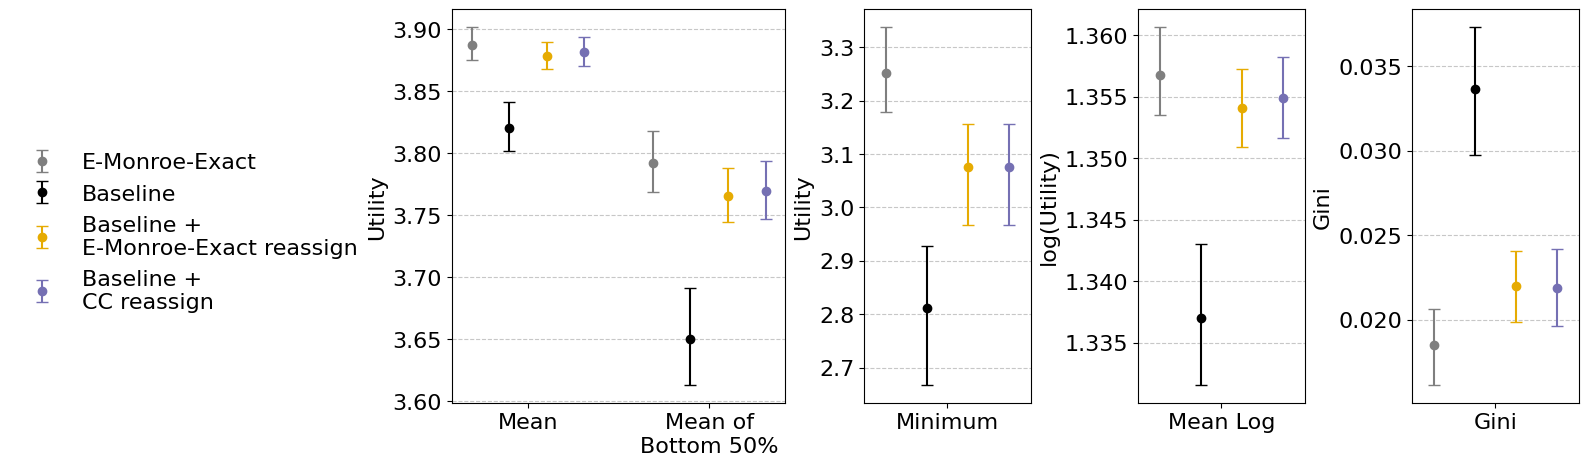
\includegraphics[width=\textwidth]{figures/voting_alg_scalar_metrics_fish_candidates.png}
  \caption{Voting algorithm SWF performance on ballot profiles generated by the baseline pipeline. Profiles are filled afterwards using additional discriminative queries. Adding either reassignment step to \Baseline{} recovers most of the performance of \EExactMonroe.}
  \label{fig:sfws-voting-algs-fish}
\end{figure*}

\subsubsection{Voting Algorithms for Expensive Discriminative Queries}
\label{sec:expensive-queries}

\Cref{fig:sfws-voting-algs-fish} compares the two algorithms for expensive discriminative queries, \Baseline{} + \EExactMonroe{} reassign and \Baseline{} + CC reassign (\Cref{sec:algorithms}), with \Baseline{} and \EExactMonroe{} on the 15 ballot profiles of the baseline pipeline.

\paragraph{Computing more of the utility matrix is the largest improvement}
Having all voters rate the baseline's slate and then reassigning them improves every SWF on every profile, except for one profile on which the minimum utility is unchanged.
\Baseline{} + \EExactMonroe{} reassign recovers 87\% of the gap between \Baseline{} and \EExactMonroe{} in mean utility (0.058 of 0.067), 81\% in bottom-50\% mean utility, and 60\% in minimum utility.
CC reassignment performs almost identically.
In our setting (\(n=100\), \(m=30\), \(k=5\)), this requires at most \(n(k-1)/2=200\) discriminative queries beyond the 1,800 used by \Baseline{}, an increase of 11\%.
The complete ballot profile requires 3,000.

Apart from the cost of greedy selection under the Monroe rule discussed above, this is the largest improvement from any single design choice we vary.
It exceeds the effect of the objective function (at most 0.018 in mean utility and 0.087 in minimum utility in \Cref{fig:sfws-voting-algs}).
It also exceeds the effect of the constituency size constraint (at most 0.008 in mean utility) and of exact rather than greedy selection under CC (at most 0.002).
The same ordering holds on the baseline's ballot profiles.
\EExactMonroe{}, which also uses the complete ballot profile to select the slate, closes the remaining gap (0.009 in mean utility, 0.18 in minimum utility).

\section{Discussion}

\subsection{Limitations} \label{sec:limitations}

\paragraph{Limited scope of evaluation}
Our case study uses a single benchmark dataset.
While its realism is an advantage over synthetic opinion distributions, for example, those used by \citet{chandak-2023}, it remains unclear how well the observed gains generalize to other domains or other distributions of opinions.
Additionally, the small sample sizes (10 runs of GenerativeCC and 15 of the baseline) may also underestimate the variance due to not sufficiently representing the population distribution of outputs for a fixed input set of opinions.

\paragraph{Virtual voters use weak LLMs}
Due to limited budget, we use GPT-4o mini for discriminative queries.
This likely introduces additional noise into the estimated ballot profile.
Although that should not systematically favor our method over the baseline, we do not perform the kind of direct human validation reported by \citet{fish-v2}.
It therefore remains possible that part of the observed improvement reflects the specifics of the models and data used here.
In general, we make no claims about the absolute alignment with human voters of the range votes made by our LLM-based virtual voters.

\paragraph{Inherited limitations from prior work}
Like \citet{fish-v2}, we do not solve broader challenges of LLM-mediated democracy, including vulnerability to jailbreaks, manipulation, and potential bias against demographic groups.
These issues remain significant obstacles to real-world deployment.

\paragraph{Non-radical Utilitarianism}
This axiom is an attempt to make a minimally restrictive illustration of a limitation of a pure utilitarian objective function.
A voting rule should not prefer to make an arbitrarily large sacrifice in other valuable SWFs for a marginal gain in total utility.
However, the choice of minimum utility as the egalitarianism SWF imposes a subjective judgment inconsistent with other choices of SWF \citep{atkinson-1970}.
There are ballot profiles, such as the example in Table~\ref{tab:egal-util-strict}, where an assignment that violates the axiom may yet be reasonably preferred on egalitarian grounds.
This axiom is overly constraining.

Additionally, none of the tested voting algorithms satisfy this axiom despite the Kolm--Pollak transformation being implemented specifically to achieve more egalitarian outcomes.
Overall, this axiom is of limited value towards its design objective of distinguishing voting algorithms that make extreme egalitarian sacrifices in optimization of a utilitarian objective.

\paragraph{Strategic voting}
Every reasonable single winner voting system with at least three candidates incentivizes strategic voting \citep{gibbards-theorem}.
\citet{rangevoting-range-voting} shows that single winner range voting achieves lower Bayesian regret than several common voting algorithms under both honest and strategic voting, across a range of synthetic ballot profile distributions.
However, \citet{preference-overstating} show that in large single winner elections, strategic voters treat range ballots as approval ballots, eliminating their expressivity advantage.
This likely extends to multiwinner elections.
Virtual voters may mitigate strategic voting, depending on how they are trained \citet{rangevoting-range-voting, newberry-moral-parliaments}.
Even if a virtual voter could be trained to report its principal's beliefs honestly, the principal is still incentivized to misrepresent her beliefs in the training data.
Ensuring virtual voter honesty is a difficult problem outside of our scope, and we simply assume that the voter opinions in the dataset that we test are honest.
Approval-style ballots may therefore remain attractive in real deployments.

\begin{table}[t]
\centering
\begin{tabular}{l|cc}
\hline
 & $a_1$ & $a_2$ \\
\hline
Voter 1 & 0.01 & 0 \\
Voter 2 & 0.01 & 1 \\
Voter 3 & 2 & 1 \\
\hline
\end{tabular}
\caption{Example ballot profile demonstrating the strictness of Egalitarian--Utilitarian Efficiency.
For \(k=1\), only \(a_1\) satisfies the axiom, while \(a_2\) may nevertheless be judged more egalitarian and preferred.}
\label{tab:egal-util-strict}
\end{table}

\subsection{Future Work}

To address the limited scope of evaluation, future work should evaluate representative slate generation systems on additional datasets such as those of \citet{gsc-next-gen} and synthetic datasets.
Work is needed to develop  better LLM-based virtual voters than our simple in-context learning methods.
Evaluations of a virtual voter's ability to represent the opinion of individual humans should also be developed.
Potential improvements to GenerativeCC itself include using more capable LLMs, Psi proportional representation voting algorithms \citep{rangevoting-optimal-pr}, and exploring the tradeoffs of approval ballots.
Insight can also be gained from human studies of representative slate generation systems.
For example, the experimental design of \citet{habermas-machine} could be adapted to use larger groups of participants, and a human validation study like that of \citet{fish-v2} could be repeated for new systems.

\section{Conclusion}

We studied representative slate generation: the task of transforming many free-form opinions into a small, weighted slate of representative statements.
The goal is not to achieve consensus in a single step, but to model  diversity in a form more flexible for its compactness.

We presented GenerativeCC, an LLM-based pipeline that combines statement generation, virtual voting, and multiwinner range voting methods to select representative statements and assign voters to them.
On the chatbot personalization benchmark, this pipeline improves on the closest prior system across all selected social welfare functions.
Ablation results suggest that the improvement is not explained solely by better clustering or by generating more candidates, but by the broader design choice of evaluating all voters against all candidates and optimizing the final slate globally.

%At the same time, the work remains exploratory.
%Our evaluation is limited to one dataset, lacks human validation, and inherits broader concerns about robustness, manipulation, and bias in virtual democracy systems.
%We nevertheless present opinion condensation as a useful subproblem for virtual democracy, and our pipeline as a starting point for focused development.
While this work remains exploratory and suffers from several limitations (see \Cref{sec:limitations}), we see representative slate generation as a useful subproblem for virtual democracy, and GenerativeCC as a starting point for focused development.

\section*{Author Contributions}

AS produced the initial idea for the project, and both authors refined it.
AS performed the literature review and contextualization of the project, as well as the selection, design, and testing of the axioms, and implemented the Monroe voting algorithm.
PB developed and implemented the other voting algorithms, did initial design of some axioms, implemented the LLM embeddings, added formal proofs, and ran the embedding and statement count ablation studies.
Both authors performed main pipeline experiments, analysis, time complexity analysis, and both wrote the paper.

\bibliography{gen_social_choice}

\appendix
% cleveref's own \appendix hook no longer fires under recent LaTeX kernels, so
% \Cref{app:...} would print "Section"; alias the sectioning counters explicitly.
\crefalias{section}{appendix}
\crefalias{subsection}{appendix}
\crefalias{subsubsection}{appendix}

\section{Embedding Ablation Study Details}
\label{app:embedding-ablation-details}

\Cref{fig:scalar-metrics-embeddings,fig:mth-happiest-embeddings} show the results of running GenerativeCC and the pipeline of \citet{fish-v2} with different embedding choices on the chatbot personalization dataset.
In both pipelines, the embeddings only determine the groups of similar voters that a subset of the statement generators are prompted with: the five clusters in GenerativeCC (\Cref{sec:statement-generation}), and the nearest neighbors found by three of the six generators of the baseline.
The improved LLM embeddings account for only a small portion of the overall difference in performance.

Both baseline series in this ablation use a slightly modified \citet{fish-v2} pipeline with a different voting algorithm due to a mistake in the experiment.
Each round of slate selection considers only the candidates generated in that round, rather than all previously generated candidates.
We expect this change to an unrelated part of the pipeline to introduce negligible bias in the comparison, so we did not rerun the experiment.

\begin{figure}[t]
  \begin{center}
  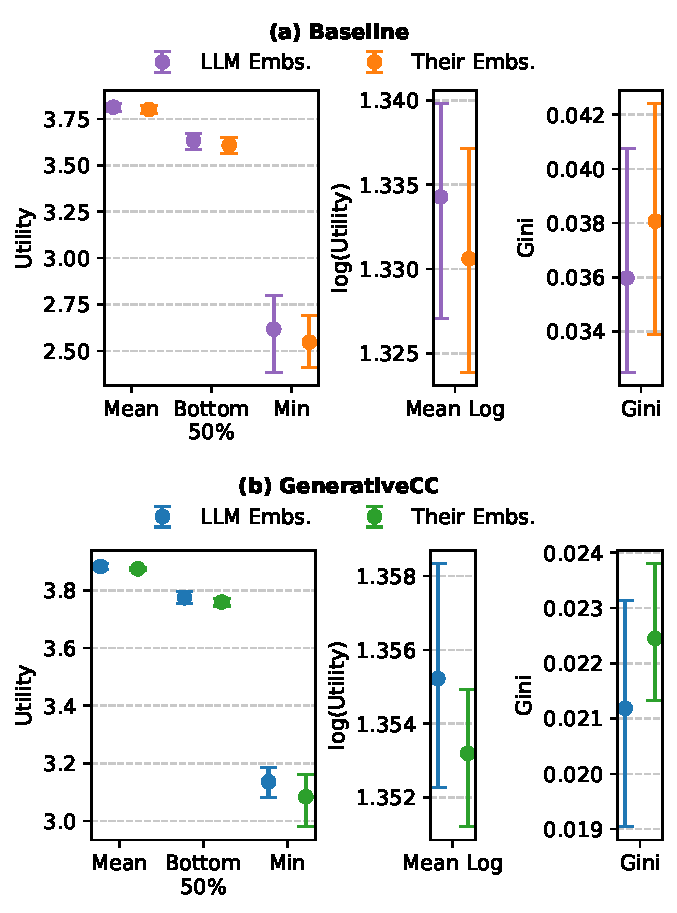
\includegraphics[width=\columnwidth]{figures/scalar_confidence_intervals_all_stacked.pdf}
  \caption{Comparison of SWF performance for an ablation changing only the embeddings in (a) the \citet{fish-v2} baseline (b) GenerativeCC. Using LLM embeddings accounts for only a small portion of the overall SWF performance difference in \Cref{fig:swf-main}.
}
  \label{fig:scalar-metrics-embeddings}
  \end{center}
\end{figure}

\begin{figure*}[t]
  \begin{center}
  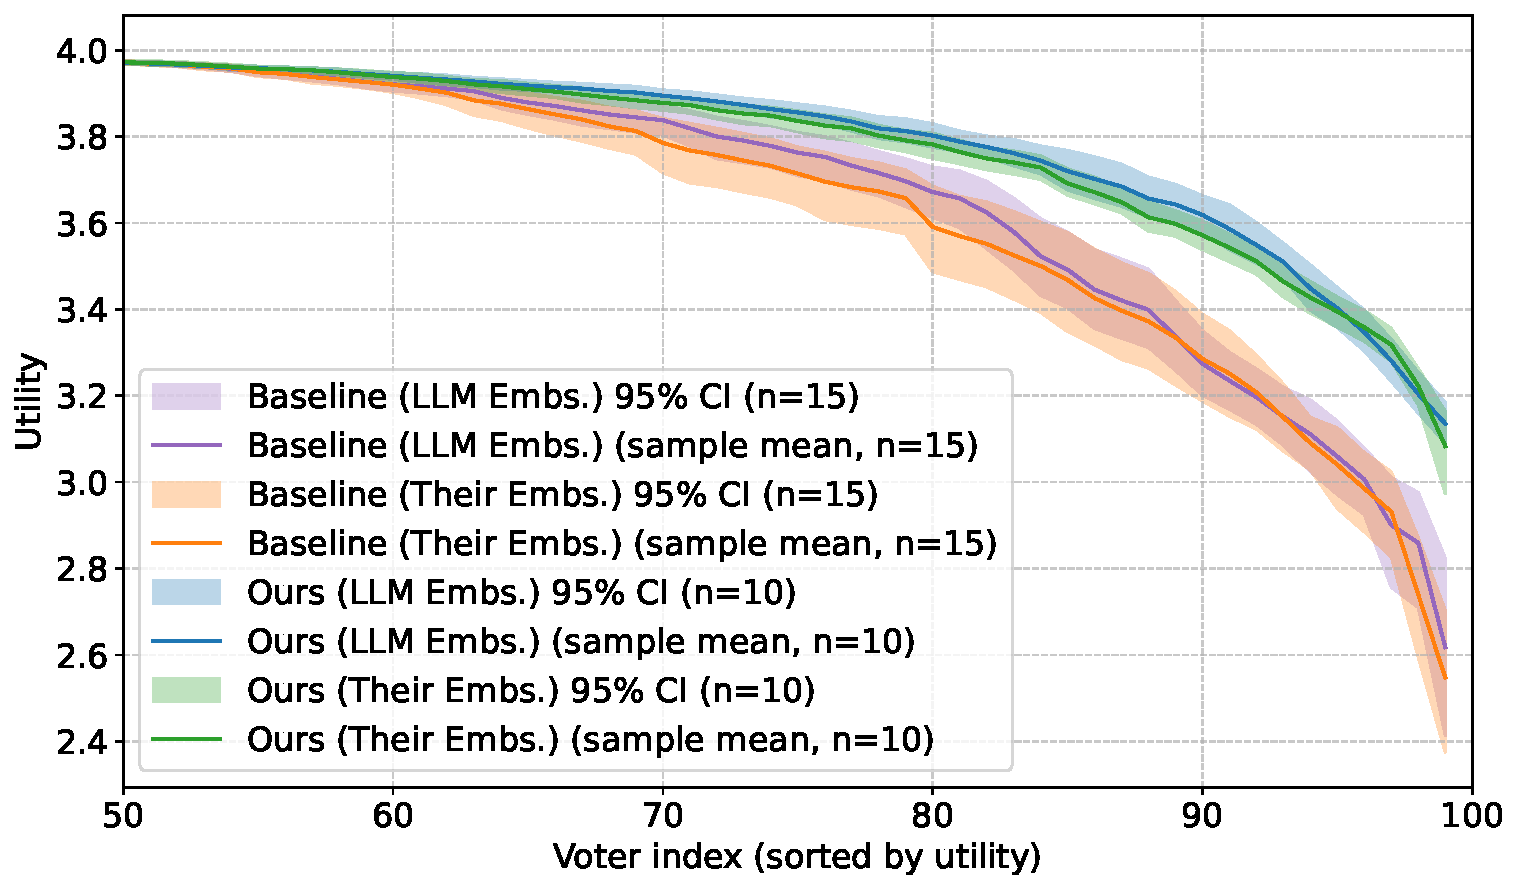
\includegraphics[width=0.8\textwidth]{figures/sorted_utility_CIs_all.pdf}
  \caption{While LLM embeddings improve utilities fairly consistently, the effect remains limited at the individual voter level.}
  \label{fig:mth-happiest-embeddings}
  \end{center}
\end{figure*}

\section{Statement Count Ablation Study Details}
\label{app:statement-ablation-details}

Because GenerativeCC generates more candidate statements than the baseline (42 vs.\ 30 in the chatbot personalization experiments), we ran an additional ablation to test whether this difference alone explains the performance gap.

In the ablated variant, we subsample the output of the generator that proposes five statements at once.
For each such call, we retain only 3 randomly selected statements and discard the remaining 2.
Since this generator is applied once to the full population and once to each of the five clusters, the total number of candidates is reduced by \(6\times 2=12\), bringing the total from 42 down to 30.

\Cref{fig:statement-ablation-comparison} compares the full GenerativeCC pipeline, the ablated pipeline, and the baseline of \citet{fish-v2}.
The ablation causes little change in performance, and the gap to the baseline remains nearly unchanged across metrics.
This supports the claim that our gains are not primarily due to a larger candidate pool.

\begin{figure*}[t]
  \begin{center}
  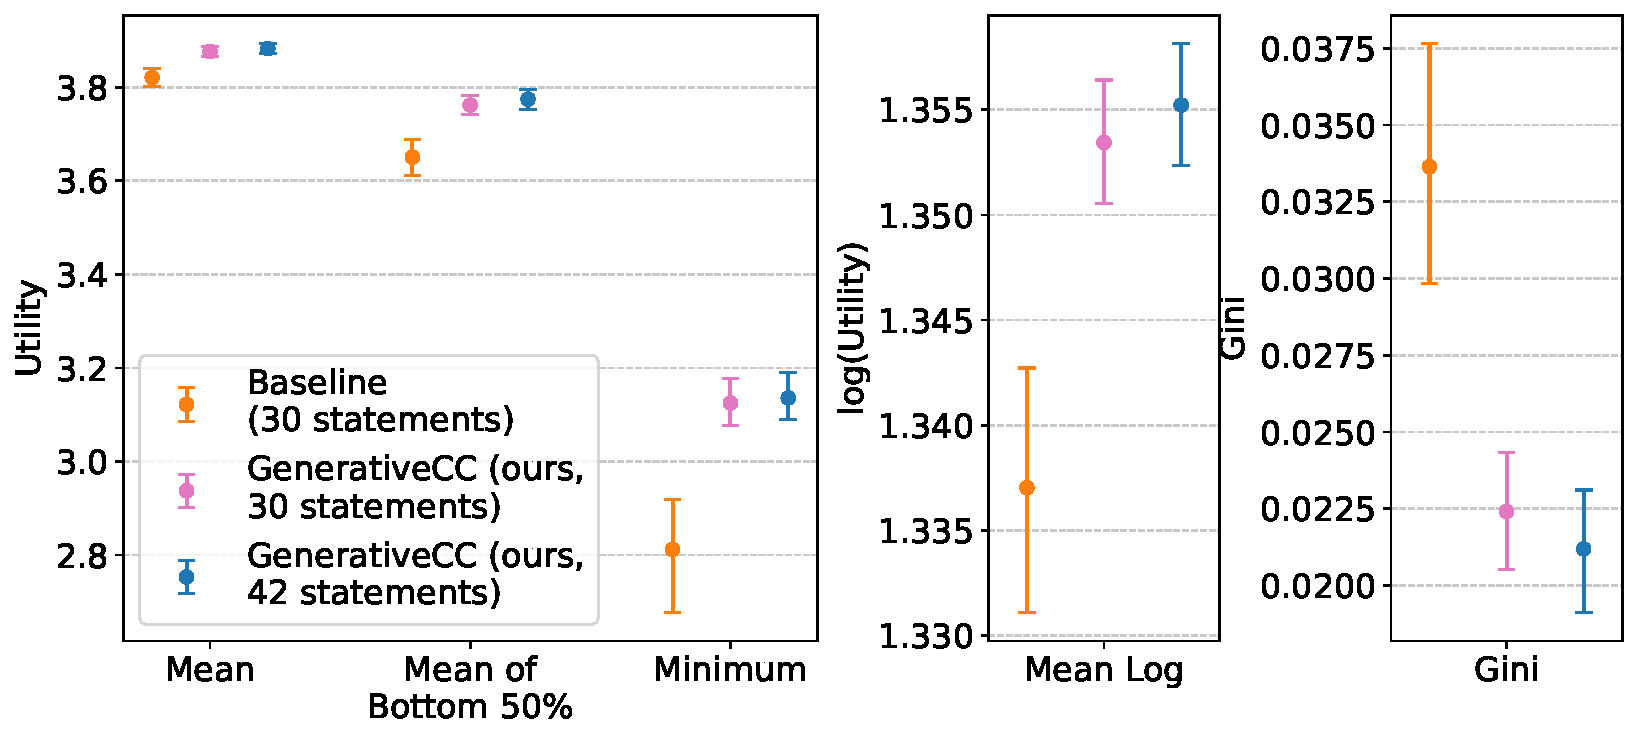
\includegraphics[width=0.8\textwidth]{figures/statement_ablation_comparison.pdf}
  \caption{Reducing GenerativeCC to the same number of generated statements as the baseline has little effect on performance.}
  % Note: Embeddings are LLM for GenerativeCC and their original one for their pipeline
  \label{fig:statement-ablation-comparison}
  \end{center}
\end{figure*}

\section{Voting Algorithm Details}

\subsection{Optimization Problems of the Exact Algorithms and \LP{}}
\label{app:exact-lp-formulations}

We solve all integer programs with PuLP/CBC \citep{pulp, john_forrest_cbc}.
At the scale of our benchmark, the solver terminates quickly, but exact worst-case complexity remains exponential.

Both \Exact{} and \LP{} are based on the same assignment-and-selection optimization problem.
Let \(x_j\) indicate whether candidate \(j\) is selected, and let \(y_{ij}\) indicate whether voter \(i\) is assigned to candidate \(j\).
\Exact{} solves
\[
\begin{aligned}
\text{maximize} \quad & \sum_i \sum_j U_{ij}\cdot y_{ij} \\
\text{subject to} \quad
& \sum_j x_j = k \\
& \sum_j y_{ij} = 1 \quad \forall i \\
& y_{ij} \le x_j \quad \forall i,j \\
& x_j \in \{0,1\} \quad \forall j \\
& y_{ij} \in \{0,1\} \quad \forall i,j.
\end{aligned}
\]

\LP{} uses the same objective and constraints, but relaxes the integrality conditions to
\[
x_j \in [0,1] \quad \forall j,
\qquad
y_{ij} \in [0,1] \quad \forall i,j.
\]

After solving the LP relaxation, we select the \(k\) candidates with highest fractional \(x_j\) values and assign each voter to their most preferred selected candidate.

\ExactMonroe{} adds the constituency-size constraints
\[
\lfloor n/k\rfloor\, x_j \;\le\; \sum_i y_{ij} \;\le\; \lceil n/k\rceil\, x_j \quad \forall j
\]
to the integer program of \Exact{}.
Each selected candidate is therefore assigned \(\lfloor n/k\rfloor\) or \(\lceil n/k\rceil\) voters, and each unselected candidate none.

The egalitarian algorithms \ECCExact{} and \EExactMonroe{} solve a sequence of integer programs with the constraints of \Exact{} and \ExactMonroe{}, respectively.
The first maximizes an auxiliary variable \(z\) subject to the additional constraints
\[
z \;\le\; \sum_j U_{ij}\, y_{ij} \quad \forall i,
\]
so its optimal value \(z^\star\) is the largest achievable minimum utility.

The remaining programs break ties leximin.
For an assignment, let \(N(t)=\sum_{i,j:\,U_{ij}\le t} y_{ij}\) be the number of voters with utility at most \(t\), and \(N^<(t)\) the number with utility below \(t\); both are linear in \(y\).
One sorted utility vector is leximin-better than another exactly when its \(N\) is smaller at the lowest threshold where the two differ.
The levels \(t_1<t_2<\cdots\) of the leximin-optimal solution are therefore found in turn.
Let \(c_0=0\), and let \(c_{l-1}\) be the number of voters at or below the levels found so far.
The next level \(t_l\) is the largest achievable \((c_{l-1}+1)\)-th lowest utility, which an integer program maximizes as \(z\) subject to \(z\le\sum_j U_{ij}y_{ij}+M w_i\) for all \(i\), with binary \(w_i\), \(\sum_i w_i\le c_{l-1}\), and \(M=\max U-\min U\).
For \(l=1\) this is the program above.
Then \(c_l\) is the smallest achievable \(N(t_l)\), which needs a second integer program only if the solution found has more than \(c_{l-1}+1\) voters at or below \(t_l\).
Every later program adds the constraints \(N^<(t_l)\le c_{l-1}\) and \(N(t_l)\le c_l\), which every leximin-optimal solution satisfies.
Each \(t_l\) is read from the utilities of the solution, rather than from the solver's objective value, to avoid losing ties to floating point error.

After each level, a feasibility program checks whether a different slate also satisfies these constraints.
If none does, the slate is leximin-optimal.
For \ECCExact{}, the search then stops, since assigning each voter to their favorite slate member is leximin-optimal for a fixed slate.
For \EExactMonroe{}, the remaining levels determine only the assignment, so the search continues with the candidates restricted to the slate.
It stops once every voter is at or below some level (\(c_l=n\)).

%\subsection{Exact vs.\ Brute-force Comparison} \label{app:brute-force-vs-exact}

%One exact way to solve the selection problem is with an integer program, which is the implementation used in our experiments.
%Another exact baseline is to enumerate all \(\binom{m}{k}\) possible slates and compute the optimal assignment for each slate directly.
%That brute-force procedure has complexity
%\[
%O\!\left(k n \binom{m}{k}\right)
%=
%O(knm^k/k!).
%\]

%We do not treat this as the worst-case complexity of the IP-based implementation.
%Rather, it is a useful comparison point: both approaches are exact, but they expose different computational bottlenecks.
%In practice, the IP solver's better average-case performance makes it far faster than exhaustive enumeration on our benchmark.

\subsection{Runtime Complexity of \Exact{}} \label{app:brute-force-vs-exact}
The \Exact{} method solves the integer program of \Cref{app:exact-lp-formulations}.
Its complexity follows from three stages: formulating the program, solving it, and extracting the assignment from the solution.

\paragraph{Problem size} The formulation has $m$ selection variables $x_j$ and $nm$ assignment variables $y_{ij}$, for $nm+m$ binary variables in total.
The constraints are one slate-size constraint, $n$ assignment constraints (one per voter), and $nm$ coupling constraints $y_{ij}\le x_j$, for $nm+n+1$ constraints in total.
Writing out the objective and these constraints therefore takes $O(nm)$ time, and reading the $O(nm)$ variable values back out to recover the slate and assignment is likewise $O(nm)$.

\paragraph{Solving} The solve step dominates.
We bound the running time of branch-and-bound with a simplex method that does not cycle, the methods CBC is built on.
CBC adds further techniques, such as presolve, cutting planes, and primal heuristics, which we do not analyze; this is one reason \Cref{tab:time-complexity} marks these bounds as solver-dependent.
Each branching step fixes one more binary variable, so the search tree has at most \(2^{nm+m+1}\) nodes.
Each node solves a linear relaxation.
The simplex method visits each basis at most once, and the number of bases is at most \(2^{V+C}\) for \(V\) variables and \(C\) constraints, with polynomial work per pivot.

The same argument applies to the other algorithms that solve integer programs.
\ExactP{} first transforms the \(nm\) utilities, which takes \(O(nm)\) time.
\ExactMonroe{} adds \(2m\) constituency-size constraints.
\ECCExact{} and \EExactMonroe{} solve at most \(3n+1\) integer programs (\Cref{app:exact-lp-formulations}), each with at most \(nm+m+n\) binary variables and a number of constraints polynomial in \(n\) and \(m\).

\paragraph{Comparison with brute force} An alternative exact baseline is to enumerate all \(\binom{m}{k}\) possible slates and compute the optimal assignment for each slate directly.
That brute-force procedure has complexity
\[
O\!\left(k n \binom{m}{k}\right).
\]
Since \(\binom{m}{k}\le m^k/k!\) and \(\binom{m}{k}\le 2^m\), it is exponential only in \(m\), and polynomial in \(n\) and \(k\).
We do not treat this as the worst-case complexity of the IP-based implementation.
Rather, it is a useful comparison point: both approaches are exact, but they expose different computational bottlenecks.
In practice, the IP solver's better average-case performance makes it far faster than exhaustive enumeration on our benchmark.

%\subsection{LP Solver Dependence on Optimization Method}
%The practical runtime of LP depends on the solver.
%Standard choices include simplex and interior-point methods.
%If one uses an interior-point method on a formulation with \(O(nm)\) variables and constraints, a standard worst-case bound is \(O((nm)^3)\).
%Our experiments use PuLP/CBC, so in the main text we describe the LP row as solver-dependent and report the interior-point bound only as a conventional reference point.

\subsection{Runtime Complexity of \LP{}}
\label{app:lp-complexity}
\LP{} uses the same formulation as \Exact{}, with the integrality constraints relaxed to $[0,1]$, so it has the same $O(nm)$ variables and $O(nm)$ constraints.
Its worst-case complexity depends entirely on which linear-programming method the solver applies.

\paragraph{Simplex (as run)} Our experiments use PuLP/CBC, which solves the relaxation with the simplex method.
Simplex runs in polynomial time on virtually every practical instance, but no polynomial worst-case bound is known for it: adversarial constructions (e.g.\ Klee--Minty cubes) force common pivot rules to visit a number of vertices exponential in the problem size.
Its running time is bounded by the number of bases, as in \Cref{app:brute-force-vs-exact}, so it is exponential in \(n\) and \(m\), as reported in \Cref{tab:time-complexity}.
Selecting the \(k\) largest fractional values and assigning each voter to their favorite selected candidate is polynomial in \(n\) and \(m\), since \(k\le m\).
As we run it, \LP{} therefore shares the same exponential worst case as \Exact{}, even though it is fast in practice.

\paragraph{Interior-point (polynomial alternative)} This exponential worst case is not inherent to the LP and can be removed by switching to an interior-point method, which runs in time polynomial in the size of the program, and therefore polynomial in \(n\) and \(m\) for utilities given to fixed precision, as ours are.
This requires only a change of solver, for example
\begin{verbatim}
# instead of the default simplex solver:
prob.solve(pulp.PULP_CBC_CMD(msg=0))

# use an interior-point solver:
prob.solve(
    pulp.GLPK_CMD(
        options=['--interior']))
# or a solver with a built-in
# interior-point method, e.g. CPLEX:
prob.solve(pulp.CPLEX_CMD())
\end{verbatim}
We decided against using this solver in our experiments because it substantially increased the runtime, even way beyond that of the exact IP solver.
It seems likely that commercial solvers lead to faster runtime.

Thus, while the \LP{} variant we benchmark has a worst case exponential in \(n\) and \(m\), an interior-point deployment is polynomial in \(n\) and \(m\) at no change to the formulation.

\subsection{Runtime Complexity of \Baseline{} + \EExactMonroe{} reassign}
\label{app:baseline-reassign-complexity}
The reassignment step runs \EExactMonroe{} on the ballot profile restricted to the baseline's slate, so it solves the integer programs of \Cref{app:exact-lp-formulations} with the slate fixed and $nk$ assignment variables.
Solved by branch-and-bound, as in our implementation, its worst-case running time is exponential in \(n\) and \(k\) and does not depend on \(m\), by the argument of \Cref{app:brute-force-vs-exact} with the \(k\) slate members in place of the \(m\) candidates.
Selecting the slate with \Baseline{} takes time polynomial in \(n\), \(m\), and \(k\), so the whole algorithm is exponential in \(n\) and \(k\) and polynomial in \(m\).
Because the slate is fixed, the reassignment can also be computed in polynomial time, as a minimum-cost flow.
In the flow network, each voter sends one unit of flow to a slate member, and each slate member receives between $\lfloor n/k\rfloor$ and $\lceil n/k\rceil$ units.
Let $v_1<\cdots<v_L$ be the distinct utilities on the slate, with $L\le nk$.
Assigning voter $i$ to slate member $j$ costs $\sum_{l:\,v_l\ge U_{ij}}(n+1)^{L-l}$, so the total cost of an assignment is $\sum_l (n+1)^{L-l} N(v_l)$, with $N$ as in \Cref{app:exact-lp-formulations}.
Since each $N(v_l)\le n$, minimizing this cost minimizes $N(v_1),N(v_2),\dots$ lexicographically, which is exactly the leximin criterion.
The costs have $O(nk\log n)$ bits, so a minimum-cost flow algorithm runs in time polynomial in $n$ and $k$, and the whole algorithm, including the slate selection, is polynomial in \(n\), \(m\), and \(k\).
The same construction computes the leximin assignment for any fixed slate, so enumerating all \(\binom{m}{k}\le 2^m\) slates gives an implementation of \EExactMonroe{} that is exponential only in \(m\), and polynomial in \(n\) and \(k\).


\section{Proofs of Axiom Satisfaction and Implications}
\label{app:axiom-proofs}
We first prove the implications among efficiency axioms stated in \Cref{sec:axioms}, then prove the axioms satisfied by \Exact{}.
Throughout, a solution is a pair $(W,\omega)$ with $|W|=k$ and $\omega:N\to W$, and $u_\omega\in\mathbb{R}_{\ge0}^n$ is the utility vector of \Cref{sec:axioms}.
As in \Cref{sec:axioms}, we assume the genericity (no-ties) condition under which each algorithm's output is unique.

\subsection{Axiom implications} \label{app:axiom-implications}
We use the dominance relations defined in \Cref{sec:axioms}, and say that an outcome satisfies the corresponding efficiency axiom when no $\omega'$ dominates it in that sense.

\paragraph{Lemma (monotone order statistics)} If $U_{i,\omega'(i)}\ge U_{i,\omega(i)}$ for all $i$, then $u_{\omega',(\ell)}\ge u_{\omega,(\ell)}$ for all $\ell$.
Using the minimax form $u_{\omega,(\ell)}=\min_{|S|=\ell}\max_{i\in S}U_{i,\omega(i)}$, every set $S$ satisfies $\max_{i\in S}U_{i,\omega'(i)}\ge\max_{i\in S}U_{i,\omega(i)}$, so the minimum over $S$ inherits the inequality.

\paragraph{Proposition 1 (Generalized Lorenz Efficiency $\Rightarrow$ Sorted Pareto Efficiency)} Suppose, for contradiction, that $\omega$ satisfies Generalized Lorenz Efficiency but violates Sorted Pareto Efficiency.
Then some $\omega'$ sorted-Pareto-dominates $u_\omega$, i.e.\ $u_{\omega',(\ell)}\ge u_{\omega,(\ell)}$ for all $\ell$, with $u_{\omega',(\ell_0)}>u_{\omega,(\ell_0)}$ for some $\ell_0$.
Grant the anonymized voter in each sorted position $\ell$ the amount $u_{\omega',(\ell)}-u_{\omega,(\ell)}\ge0$; these grants turn $u_\omega$ into $u_{\omega'}$, and the grant at $\ell_0$ is positive, so the series is non-empty.
Hence $u_{\omega'}$ generalized-Lorenz-dominates $u_\omega$, contradicting Generalized Lorenz Efficiency.

\paragraph{Proposition 2 (Sorted Pareto Efficiency $\Rightarrow$ Individual Pareto Efficiency)} Suppose, for contradiction, that $\omega$ satisfies Sorted Pareto Efficiency but violates Individual Pareto Efficiency.
Then some $\omega'$ Pareto-dominates $u_\omega$: $U_{i,\omega'(i)}\ge U_{i,\omega(i)}$ for all $i$, with at least one strict inequality and hence strictly greater total utility.
By the Lemma, $u_{\omega',(\ell)}\ge u_{\omega,(\ell)}$ for all $\ell$; since sorting preserves the sum, the strictly greater total forces $u_{\omega',(\ell)}>u_{\omega,(\ell)}$ for some $\ell$.
Hence $u_{\omega'}$ sorted-Pareto-dominates $u_\omega$, contradicting Sorted Pareto Efficiency.

\subsection{\Exact{}} \label{app:exact-axiom-proofs}
\Exact{} returns the slate $W^\star$ maximizing total utility $T(W):=\sum_i\max_{j\in W}U_{ij}$, assigning each voter to a best member of $W^\star$; let $T^\star=T(W^\star)$.

\paragraph{Independence of Common Scale} For $c>0$, replacing $U$ by $cU$ replaces $T(W)$ by $cT(W)$ for every $W$, preserving the maximizer; positive scaling also preserves each voter's within-slate preference order, so $\omega$ is unchanged.

\paragraph{Symmetry} $T$ is built from sums and maxima of utility entries, so relabeling voters or candidates permutes the set of optimal solutions identically.
Under genericity this set is a singleton: the optimal slate is unique, as is each voter's best candidate within it (assumption in \Cref{sec:axioms}).
Any correct exact solver returns this unique optimum, and with no alternative optima the result cannot depend on the solver's internal ordering of variables or constraints; only the same tie cases already excluded by the axiom could introduce such dependence.
Hence permuting $U$ permutes the output identically, leaving $\omega$ unchanged as a map.

\paragraph{Monotonicity} If $a\in W^\star$ and we raise $U_{ia}$, then $T$ is unchanged on slates omitting $a$ and weakly increased on $W^\star$, so $W^\star$ still beats every $a$-free slate and any slate beating it contains $a$; thus $a$ stays a winner.
If $a\notin W^\star$ and we lower $U_{ia}$, then $T(W^\star)$ is unchanged while every slate containing $a$ weakly decreases, so $a$ stays a loser.

\paragraph{Egalitarian--Utilitarian Efficiency} No solution exceeds $T^\star$ in total utility, so none has both greater total and greater minimum utility.

\paragraph{Generalized Lorenz Efficiency} The final Lorenz ordinate $L_n$ equals total utility.
A solution generalized-Lorenz-dominating $\omega^\star$ would have $L_n\ge T^\star$: if strict, its total exceeds $T^\star$, which is impossible; if equal, it ties $T^\star$, so there is another assignment with equal total utility which is impossible by assumption (\Cref{sec:axioms}).
Hence no dominator exists.
By Propositions 1 and 2, Sorted Pareto Efficiency and Individual Pareto Efficiency follow.


%\subsection{Monroe}
%All three Monroe variants select the same slate by the greedy procedure of \Cref{sec:voting-algorithms} and differ only in their final voter assignment.
%The selection scores each remaining candidate $c$ by an order statistic (the $\lceil n/k\rceil$-th highest utility) of the column $U_{\cdot c}$ restricted to the currently unassigned voters, adds the maximizer to the slate, and assigns its constituency by sorting those voters' utilities for $c$.
%Below we prove the axioms marked \Pass{} for all three variants.

%\paragraph{Independence of Common Scale.} For $c>0$, replacing $U$ by $cU$ multiplies every utility entry by $c$.
%Order statistics, sorts, and $\arg\max$/$\arg\min$ are all invariant under a common positive rescaling, so the greedy selection makes identical choices and forms identical constituencies; hence the slate and the greedy ($\mathrm{equal,greedy}$) and favorite-member ($\mathrm{free,greedy}$) assignments are unchanged.
%For $\mathrm{equal,optimal}$, the assignment objective $\sum_i U_{i,\omega(i)}$ is scaled by $c$ over the same feasible balanced assignments, preserving the maximizer.
%Within-constituency preference orders are likewise preserved, so $\omega$ is unchanged in every variant.

%\paragraph{Symmetry.} Every quantity used by the selection (order statistics of utility columns, sorts of utility values) and by each assignment rule depends only on utility values, not on voter or candidate labels.
%Relabeling the rows or columns of $U$ therefore permutes the selected slate and assignment identically, leaving $\omega$ unchanged as a map (unique under the genericity assumption).


\section{Reasoning and Counterexample Ballot Profiles for Axiom Failures}
\label{app:voting-failures}

\Cref{tab:failure-exact-nru,tab:failure-exactp-nru,tab:failure-greedy-indiv-pareto,tab:lp-fractional,tab:lp-monotonicity} provide representative counterexamples for the observed axiom failures discussed in the main text.
Table~\ref{tab:egal-util-strict} illustrates that Egalitarian--Utilitarian Efficiency may be overly strict in some cases.

\begin{table}[t]
\centering
\begin{tabular}{l|ccc}
\hline
 & $a_1$ & $a_2$ & $a_3$ \\
\hline
Voter 1 & 3 & 0 & 4 \\
Voter 2 & 3 & 3 & 0 \\
Voter 3 & 0 & 2 & 0 \\
\hline
\end{tabular}
\caption{Greedy Total Utility Maximization fails Individual Pareto Efficiency for $k=2$.
The selected slates include \(a_1\), while the only slate satisfying the axiom is \(\{a_2,a_3\}\).}
\label{tab:failure-greedy-indiv-pareto}
\end{table}

\subsection{\Exact{} fails Non-radical Utilitarianism}
\label{app:exact-nru}

Because \Exact{} maximizes total utility alone, it can prefer a slate with only slightly higher total utility even when an alternative offers a much larger improvement in minimum utility.
\Cref{tab:failure-exact-nru} gives a simple counterexample for \(k=1\).

\begin{table}[t]
\centering
\begin{tabular}{l|cc}
\hline
 & $a_1$ & $a_2$ \\
\hline
Voter 1 & $4$ & $8/3-\eta$ \\
Voter 2 & $4$ & $8/3-\eta$ \\
Voter 3 & $0$ & $8/3-\eta$ \\
\hline
\end{tabular}
\caption{\Exact{} fails Non-radical Utilitarianism for \(k=1\), for any sufficiently small \(\eta>0\).}
\label{tab:failure-exact-nru}
\end{table}

\Exact{} selects \(a_1\) because its total utility is
\[
4+4+0=8,
\]
while \(a_2\) has total utility
\[
3\left(\frac{8}{3}-\eta\right)=8-3\eta.
\]
However, the minimum utility under \(a_1\) is \(0\), whereas under \(a_2\) it is
\[
\frac{8}{3}-\eta.
\]
Thus, moving from \(a_1\) to \(a_2\) sacrifices only
\[
\delta=3\eta
\]
in total utility while improving the minimum utility by
\[
\epsilon=\frac{8}{3}-\eta.
\]
The ratio
\[
\frac{\epsilon}{\delta}
=
\frac{\frac{8}{3}-\eta}{3\eta}
\]
can be made arbitrarily large by taking \(\eta\) arbitrarily small.
Therefore, \Exact{} violates Non-radical Utilitarianism.

\subsection{\ExactP{} fails Non-radical Utilitarianism}
\label{app:exactp-nru}
% Example found by Claude Opus 4.7

The Kolm--Pollak transformation does not repair this failure.
\ExactP{} maximizes the \emph{transformed} total $\sum_i f(U_{i,\omega(i)})$, and because $f$ is concave it can still reject an alternative slate that is essentially tied in raw total utility but substantially better in raw minimum utility.
\Cref{tab:failure-exactp-nru} gives a counterexample for $k=1$ and $\kappa=\ln 1.5$, where $\delta>0$ is a free parameter.
\begin{table}[t]
\centering
\begin{tabular}{l|cc}
\hline
 & $a_1$ & $a_2$ \\
\hline
Voter 1 & $0$   & $1/2$ \\
Voter 2 & $5/2$ & $1/2$ \\
Voter 3 & $5/2$ & $4-\delta$ \\
\hline
\end{tabular}
\caption{Counterexample showing that \ExactP{} fails Non-radical Utilitarianism for \(k=1\) and \(\kappa=\ln 1.5\), for any sufficiently small \(\delta>0\).}
\label{tab:failure-exactp-nru}
\end{table}
For \(\kappa=\ln 1.5\) the transformation is \(f(u)=3\bigl(1-1.5^{-u}\bigr)\), giving
\[
f(0)=0,\quad f(\tfrac12)\approx0.55,
\]
\[
f(\tfrac52)\approx1.91,\quad f(4)\approx2.41
\]
\ExactP{} selects the slate with the larger transformed total.
For \(a_1\),
\[
f(0)+2f(\tfrac52)\approx3.83,
\]
while for \(a_2\), using \(f(4-\delta)\le f(4)\) since \(f\) is increasing,
\[
2f(\tfrac12)+f(4-\delta)\;\le\;2f(\tfrac12)+f(4)\approx3.51
\]
The bound holds for every \(\delta\ge 0\), so \ExactP{} selects \(a_1\).

The raw total utilities are
\[
\underbrace{0+\tfrac52+\tfrac52}_{a_1}=5,\qquad
\underbrace{\tfrac12+\tfrac12+(4-\delta)}_{a_2}=5-\delta,
\]
and the raw minimum utilities are \(0\) under \(a_1\) and \(1/2\) under \(a_2\).
Moving from \(a_1\) to \(a_2\) therefore sacrifices only \(\delta\) in total utility while improving the minimum utility by \( \epsilon=\tfrac12 .\)
The ratio \(\epsilon/\delta = 1/(2\delta)\) can be made arbitrarily large by taking \(\delta\) arbitrarily small.
Therefore \ExactP{} violates Non-radical Utilitarianism.

The same profile is a counterexample for every \(\kappa>0\), hence \ExactP{} fails Non-radical Utilitarianism for all \(\kappa>0\).
This is expected of any scalar inequality-averse objective: an arbitrarily large \(\epsilon/\delta\) tradeoff amounts to lexicographic priority for the worst-off voter, which is instead obtained by lexicographic maximin optimization \citep{luss-1999, kostreva-ogryczak-wierzbicki-2004}.
%, and in particular in the limit \(p\to1^{+}\).
%counterexamples for larger \(p\) follow from the same mechanism (a steep region of \(f\) amplifying several small per-voter losses) and can be located by adversarial search.
%Hence Exact$(p>1)$ fails Non-radical Utilitarianism for all \(p>1\).

\subsection{\ExactP{} fails Independence of Common Scale}
\label{app:exactp-ics}

This failure is a known property of the Kolm--Pollak EDE \citep{kolm-1976, blackorby-donaldson-1980}.
A counterpart to this EDE is the Atkinson family \citep{atkinson-1970}, which satisfies Independence of Common Scale, but fails a similar axiom of Independence of Common Shift: adding a constant to all utilities never changes $\omega$.
\ExactP{} satisfies this axiom \citep{blackorby-donaldson-1980}.

\subsection{Worst-Case Behavior of \LP{}}
\label{app:lp-worst}

Unlike \Exact{}, the LP relaxation can have a \emph{strictly fractional} optimum.
The subsequent rounding step of selecting the $k$ candidates with the largest $x_j$ is then sensitive both to the tie-breaking rule and to small perturbations of the ballot profile.
Importantly, if the fractional optimum assigns equal weights to all statements, \LP{} does not provide any useful information and can end up selecting the worst possible slate.

\begin{table}[t]
\centering
\begin{tabular}{l|cccc}
\hline
 & $a_1$ & $a_2$ & $a_3$ & $a_4$ \\
\hline
Voter 1 & 3.61 & 3.45 & 0.47 & 1.78 \\
Voter 2 & 2.32 & 0.53 & 0.38 & 1.74 \\
Voter 3 & 0.37 & 3.06 & 1.72 & 3.37 \\
Voter 4 & 1.09 & 0.39 & 3.97 & 2.19 \\
\hline
\end{tabular}
\caption{Profile with $k=2$ whose LP relaxation has a strictly fractional optimum.
\LP{} selects $\{a_1,a_2\}$, which is Pareto-dominated by $\{a_1,a_4\}$.}
\label{tab:lp-fractional}
\end{table}

\Cref{tab:lp-fractional} gives a profile with $k=2$ that exhibits this behavior.
For this profile every integral $2$-slate has total utility at most $11.62$ (attained by $\{a_1,a_3\}$), whereas the fractional point $x=(\tfrac12,\tfrac12,\tfrac12,\tfrac12)$ attains $11.855$: each voter then receives half of each of their two highest utilities.
The LP optimum is therefore this fully symmetric fractional point.
Because all $x_j$ are equal, the rounding step breaks ties by candidate order and returns $\{a_1,a_2\}$, with utility vector $(3.61,2.32,3.06,1.09)$.

This slate is Pareto-dominated by $\{a_1,a_4\}$, whose utility vector $(3.61,2.32,3.37,2.19)$ is weakly larger for every voter and strictly larger for voters 3 and 4.
Hence \LP{} violates Individual Pareto Efficiency, and therefore also Sorted Pareto Efficiency and Generalized Lorenz Efficiency (and Egalitarian--Utilitarian Efficiency, since $\{a_1,a_4\}$ has both higher total and higher minimum utility).
The same example shows why \LP{} violates Symmetry: the optimal $x$ is invariant under relabeling the candidates, so the selected slate is fixed entirely by the tie-breaking rule, and relabeling the candidates changes the outcome.

\LP{} also fails Monotonicity.
\Cref{tab:lp-monotonicity} gives a profile, again with $k=2$, for which the LP optimum is initially integral, $x=(0,1,1,0)$, so \LP{} selects $\{a_2,a_3\}$.
Now increase voter 1's rating of the winning candidate $a_3$ from $0.04$ to $1.5$.
This lifts the value of the symmetric fractional point above that of every integral slate ($11.46$ versus $11.33$), so the LP optimum becomes $x=(\tfrac12,\tfrac12,\tfrac12,\tfrac12)$ and rounding returns $\{a_1,a_2\}$.
The candidate $a_3$ is dropped from the winning slate even though a voter's rating of it \emph{increased}; hence \LP{} violates Monotonicity.

\begin{table}[t]
\centering
\begin{tabular}{l|cccc}
\hline
 & $a_1$ & $a_2$ & $a_3$ & $a_4$ \\
\hline
Voter 1 & 1.14 & 2.05 & 0.04 & 0.68 \\
Voter 2 & 3.09 & 3.45 & 0.72 & 0.71 \\
Voter 3 & 3.68 & 0.11 & 3.60 & 0.17 \\
Voter 4 & 0.05 & 1.02 & 2.23 & 3.32 \\
\hline
\end{tabular}
\caption{Profile with $k=2$ showing that \LP{} fails Monotonicity.
As shown, the LP optimum is integral and \LP{} selects $\{a_2,a_3\}$.
Raising $U_{1,a_3}$ from $0.04$ to $1.5$ makes the LP optimum the fractional point $x_j=\tfrac12$, after which \LP{} selects $\{a_1,a_2\}$: the winning candidate $a_3$ is dropped despite an increase in its rating.}
\label{tab:lp-monotonicity}
\end{table}

%All three failures share one mechanism: when the LP relaxation has a fractional optimum, the integral slate is determined by the rounding and tie-breaking rules rather than by the utilities directly, which makes the outcome discontinuous in the ballot profile and dependent on candidate labels.

%\subsection{Worst-Case Behavior of LP}

%\begin{table}[t]
%\centering
%\begin{tabular}{l|cccc}
%\hline
% & $a_1$ & $a_2$ & $a_3$ & $a_4$ \\
%\hline
%Voter 1 & 0.1003 & 0.2004 & 4.1001 & 2.0002 \\
%Voter 2 & 9.0005 & 8.9006 & 1.0007 & 1.1008 \\
%Voter 3 & 6.0011 & 7.0009 & 1.2002 & 7.1001 \\
%Voter 4 & 8.0013 & 7.9014 & 1.3005 & 1.4006 \\
%\hline
%\end{tabular}
%\caption{Example where the LP relaxation treats all four candidates symmetrically when \(k=2\).}
%\label{tab:lp-worst-case}
%\end{table}

%For the profile in \Cref{tab:lp-worst-case}, an optimal solution to the LP relaxation assigns \(x_j=0.5\) to every candidate.
%Our rounding scheme then breaks ties by candidate order and picks the first two statements, yielding \(\{a_1,a_2\}\).
%But that slate is Pareto-dominated by \(\{a_1,a_4\}\), so Individual Pareto Efficiency fails.
%This example also shows why LP can violate symmetry with respect to candidate order: once the relaxation has flattened distinctions between candidates, the final outcome depends on the tie-breaking rule.

\section{Contributions of Generators}
\label{app:statement-origin}

This appendix reports which statement-generation methods contributed the finally selected statements in GenerativeCC.

\subsection{Statement Origin in GenerativeCC}

Across ten runs, we generate a slate of 5 statements per run, for a total of 50 selected statements.
Aggregating across runs, the selected statements were generated by:
\begin{itemize}
    \item %\texttt{NamedChatbotPersonalizationGenerator} (cluster of voters): 21
Single-statement generator (on clusters of voters): 21
    \item Batch generator (on clusters of voters): 19
    \item Single-statement generator (on all voters): 5
    \item Batch generator (on all voters): 5
\end{itemize}

These counts show that all generation modes contribute to the final slates rather than one method dominating completely.
(For description of generation methods, refer to \Cref{sec:statement-generation}.)


\section{Confounding Variable Analysis}
\label{app:model-drift}

This appendix examines whether model drift or differences in line endings could affect our results.
\Cref{tab:confounder-systems} summarizes which results are potentially affected.
The GenerativeCC runs and the earlier baseline runs (\Cref{app:embedding-ablation-details}) were produced between May and August 2025, while
the baseline runs of \Cref{fig:swf-main,fig:mth-happiest-main} are from 2026.
Due to the long interval between their LLM calls, there is an elevated risk of model drift confounding comparisons.
Additionally, the baseline data in \Cref{fig:scalar-metrics-embeddings,fig:mth-happiest-embeddings} was generated using CRLF line endings in some prompts rather than LF line endings.
If line endings meaningfully affect the behavior of LLM elements of the pipeline, this could also be a confounder.

\begin{table*}[t]
\centering
\begin{tabular}{llll}
\hline
System & Results & LLM calls made & Line endings \\
\hline
GenerativeCC & all & May--Aug.\ 2025 & LF \\
Baseline & \Cref{fig:swf-main,fig:mth-happiest-main,fig:sfws-voting-algs,fig:statement-ablation-comparison} & 2026 & LF \\
Baseline & \Cref{fig:scalar-metrics-embeddings,fig:mth-happiest-embeddings} & May--Aug.\ 2025 & CRLF \\
\hline
\end{tabular}
\caption{The timing of each system's LLM calls, and the line endings of their prompts.}
\label{tab:confounder-systems}
\end{table*}

\subsection{Model drift}
\label{app:drift}

Even a fixed model snapshot served through an API can behave differently over time, for example through changes to the serving infrastructure \citep{anthropic2025postmortem}; the performance of \texttt{gpt-4o-2024-08-06}, our generator, has been shown to vary with the time of day and week \citep{tschisgale2026periodicity}.
OpenAI may thus have changed how our snapshots are served between 2025 and 2026, introducing model drift.
We test whether an LLM call made in 2026 behaves like one more call from 2025, for every type of call whose outputs enter a comparison between the two periods.
Each sampled 2025 call is repeated in 2026.

\paragraph{Reference: variance within 2025.}
Since the models are nondeterministic, we compare the differences between 2025 and 2026 outputs with the differences between 2025 outputs of the same prompt.
For ratings of candidate statements, such repeated prompts are rare: only four candidate statements appear in more than one of the 15 earlier baseline runs, giving 400 (voter, statement) cells rated twice.
\textbf{Four statements are too few to measure the variance of these ratings.}
For nearest-neighbor searches, 1{,}453 (voter, summary) pairs, covering 33 summaries, were rated in two different runs.
For generation, three of the baseline's generators received identical inputs in the first round of all 15 runs: the two prompted with the opinions of all voters, at temperatures 0 and 1, and the one prompted with a random subsample of five opinions, which is the same in every run.
We measure the variance of each one's 15 outputs by their mean pairwise cosine distance between \texttt{text-embedding-3-small} embeddings, a proxy measurement of the semantic variance among generated statements (2025 rows of \Cref{tab:model-drift-generation}).

\paragraph{Discriminative queries.}
We create three samples of 2025 rating calls and repeat them in 2026:
\begin{itemize}
    \item \emph{Baseline candidates} (300 ratings): ratings of candidate statements in the 15 earlier baseline runs, covering all six generators and all five rounds.
    The sample consists of 100 of the 400 cells rated twice in 2025, and 200 further cells, 50 from each bin of the 2025 rating (\(<2\), \(2\)--\(3\), \(3\)--\(3.5\), \(>3.5\)).
    \item \emph{GenerativeCC candidates} (192 ratings): cells of the 10 GenerativeCC utility matrices, stratified by the same bins.
    \item \emph{Nearest-neighbor search} (152 ratings): the baseline's calls rating another voter's summary, parsed from the logs of the earlier baseline runs and stratified by the same bins.
\end{itemize}
The calls of the earlier baseline runs are repeated with their CRLF line endings, and those of GenerativeCC with LF (\Cref{tab:confounder-systems}).
Equal numbers of ratings per bin do not match the distribution of 2025 ratings: among all 27{,}000 ratings of candidate statements in the 15 earlier baseline runs, 49\% are above \(3.5\) and 2\% below \(2\), whereas among all 10{,}275 logged nearest-neighbor searches, 33\% are below \(2\).
We therefore compute each estimate as a weighted average of its values within the bins, weighting each bin by its share of all 2025 ratings of the same type, so that estimates describe all 2025 ratings of a type rather than the sample.

\Cref{tab:model-drift-ratings} shows the bias, the mean difference between the 2026 and 2025 ratings, with 95\% bootstrap confidence intervals from 2{,}000 resamples.
\textbf{None of the three types of ratings shows a detectable bias.}

\begin{table}[t]
\centering
\begin{tabular}{lcc}
\hline
Rating type & \(n\) & \makecell{Bias\\(95\% CI)} \\
\hline
\makecell[l]{Baseline\\candidates} & 300 & \makecell{\(+0.002\)\\\([-0.017, +0.021]\)} \\
\hline
\makecell[l]{GenerativeCC\\candidates} & 192 & \makecell{\(-0.005\)\\\([-0.026, +0.018]\)} \\
\hline
\makecell[l]{Nearest-neighbor\\search} & 152 & \makecell{\(+0.031\)\\\([-0.019, +0.084]\)} \\
\hline
\end{tabular}
\caption{Bias: mean difference between 2026 ratings repeating 2025 calls and the original 2025 ratings (2026 \(-\) 2025), on the \(0\)--\(4\) scale, weighted to the population distribution of 2025 ratings, with 95\% bootstrap confidence intervals.}
\label{tab:model-drift-ratings}
\end{table}

\textbf{For ratings of candidate statements, we therefore cannot tell whether the variance of the ratings changed.}
For nearest-neighbor searches, whose reference covers 33 summaries, we compare variances by the \emph{spread ratio}: the mean squared difference between the 2026 and 2025 ratings divided by that between two 2025 ratings, combined over bins with population weights.
A ratio of \(1\) means that a 2026 rating varies around a 2025 rating exactly as much as another 2025 rating would.
The ratio is \(2.03\), with a 95\% confidence interval of \([1.05, 3.62]\) from resampling the rated summaries, since ratings of the same summary are not independent.
So \textbf{2026 nearest-neighbor searches have higher variance than 2025 ones}.

\paragraph{Generative queries.}
We use two sets of 2026 generation calls.
First, we repeat the first-round calls of the three generators with identical first-round inputs 15 times each, with the exact 2025 messages and parameters, and compare their outputs with the 15 outputs of 2025 by cosine distance.
Second, we repeat 24 logged generation calls of the 2025 runs, four from each of the six generators of the baseline, spread over rounds, each twice with the exact logged messages and parameters (48 calls).
Since most of these calls have only one 2025 output, we use them only to compare quality and format: six fixed voters rate each 2025 output and both 2026 outputs, with all ratings made in 2026 so that drift of the rater cancels.

\begin{table}[t]
\centering
\begin{tabular}{lcc}
\hline
Calls made & CRLF & LF \\
\hline
\multicolumn{3}{l}{\emph{All voters, temperature 0}} \\
2025 & \(0.139\) & \\
2026 & \(0.004\) & \(0.006\) \\
\hline
\multicolumn{3}{l}{\emph{All voters, temperature 1}} \\
2025 & \(0.148\) & \\
2026 & \(0.145\) & \(0.089\) \\
\hline
\multicolumn{3}{l}{\emph{Subsample of five voters}} \\
2025 & \(0.024\) & \\
2026 & \(0.016\) & \(0.016\) \\
\hline
\end{tabular}
\caption{Variance of the first-round outputs of the three generators with identical first-round inputs in every run: mean pairwise cosine distance between the embeddings of 15 outputs (30 for 2026 LF), by the year of the calls and the line endings of their prompts. The 2025 outputs come from the earlier baseline runs, and 15 of the 2026 LF outputs from the baseline runs of \Cref{fig:swf-main,fig:mth-happiest-main}. Blank cells have no outputs.}
\label{tab:model-drift-generation}
\end{table}

\begin{table*}[t]
\centering
\begin{tabular}{lccccc}
\hline
& \multicolumn{2}{c}{Variance} & Mean distance & \multicolumn{2}{c}{\(p\)} \\
Generator & 2025 & 2026 & between groups & Variance & Bias \\
\hline
All voters, temperature 0 & \(0.139\) & \(0.004\) & \(0.104\) & \(<0.001\) & \(<0.001\) \\
All voters, temperature 1 & \(0.148\) & \(0.145\) & \(0.144\) & \(0.93\) & \(0.92\) \\
Subsample of five voters & \(0.024\) & \(0.016\) & \(0.021\) & \(0.007\) & \(0.12\) \\
\hline
\end{tabular}
\caption{Tests of drift between 2025 and 2026 in the first-round outputs of \Cref{tab:model-drift-generation} with CRLF prompts, 15 outputs per group. \emph{Variance}: mean pairwise cosine distance within a group. \emph{Mean distance between groups}: mean distance between a 2026 output and a 2025 output. \emph{Variance \(p\)}: two-sided permutation test of whether the two variances differ. \emph{Bias \(p\)}: two-sided permutation test of whether the mean distance between groups differs from the variance of the 2025 outputs, which it would not if the outputs of the two groups were exchangeable. All tests use 20{,}000 permutations of the group labels.}
\label{tab:model-drift-generation-tests}
\end{table*}

\begin{table*}[t]
\centering
\begin{tabular}{lccccc}
\hline
& \multicolumn{2}{c}{Variance} & Mean distance & \multicolumn{2}{c}{\(p\)} \\
Generator & CRLF & LF & between groups & Variance & Bias \\
\hline
All voters, temperature 0 & \(0.004\) & \(0.006\) & \(0.006\) & \(0.003\) & \(0.006\) \\
All voters, temperature 1 & \(0.145\) & \(0.089\) & \(0.123\) & \(0.050\) & \(0.13\) \\
Subsample of five voters & \(0.016\) & \(0.016\) & \(0.027\) & \(0.88\) & \(0.002\) \\
\hline
\end{tabular}
\caption{Tests of line endings, CRLF vs.\ LF, in the 2026 first-round outputs of \Cref{tab:model-drift-generation}, with 15 CRLF and 30 LF outputs per generator. Columns as in \Cref{tab:model-drift-generation-tests}, with CRLF in place of 2025: the bias test compares the mean distance between groups with the variance of the CRLF outputs.}
\label{tab:line-endings-generation-tests}
\end{table*}

\Cref{tab:model-drift-generation} shows the variance of the first-round outputs, and \Cref{tab:model-drift-generation-tests} the tests of drift.
\begin{itemize}
    \item \emph{Variance among runs.}
    \textbf{Generation has much lower variance among runs in 2026 than in 2025 at temperature 0, and somewhat lower variance for the subsampling generator}, with the prompts held fixed.
    At temperature 1, we detect no difference (\(0.145\) vs.\ \(0.148\), \(p = 0.93\)).
    \item \emph{Bias.}
    With the prompts held fixed, the 2026 outputs are no farther from the 2025 outputs than 2025 outputs are from each other for any generator, and at temperature 0 they are closer.
    The lower variance of 2026 outputs explains why they can be closer: outputs concentrated among the 2025 outputs are closer to them on average than these are to each other.
    So \textbf{the 2026 output distribution lies within the spread of the 2025 output distribution}.
    It's possible that the 2026 distribution is biased relative to the 2025 distribution, where the 2026 distribution lies mostly inside the 2025 distribution, but the sample sizes are too small to detect this.
    \item \emph{Quality.}
    Mean agreement with 2026 outputs differs from that with 2025 outputs by \(+0.06\) \([-0.02, +0.16]\), with \textbf{no detectable bias}.
    Two 2026 outputs of the same prompt differ by \(0.06\) on average.
    \item \emph{Format.}
    \textbf{The mean response lengths are similar} (71--86 words per generator in 2025, 71--85 in 2026).
\end{itemize}

\subsection{Line endings}
\label{app:line-endings}

All results in the paper use prompts with LF line endings, except the two baseline series of the embedding ablation (\Cref{fig:scalar-metrics-embeddings,fig:mth-happiest-embeddings}), whose runs used CRLF.

\paragraph{Ratings.}
A rating prompt contains a voter's opinion and the rated statement.
We re-rate 40 cells of the GenerativeCC utility matrices, 10 from each utility bin, in 2026 with each combination of line endings in the opinion and in the statement.
All-LF prompts reproduce the 2025 ratings best, with a bias of \(-0.002\) \([-0.047, +0.044]\) and a mean absolute difference of \(0.085\), compared with \(0.116\) to \(0.159\) for the other combinations, so we infer that GenerativeCC used LF.
A second sample of 120 cells of the GenerativeCC variant with the embeddings of \citet{fish-v2}, rated with all-CRLF and all-LF prompts, gives the same result, with mean absolute differences of \(0.100\) for LF and \(0.114\) for CRLF.
Prompts formatted as in the earlier baseline runs, with CRLF opinions and LF statements, rate \textbf{\(0.073\) \([0.010, 0.134]\) higher than all-LF prompts}, weighted to the distribution of GenerativeCC ratings; the difference is largest for ratings below \(2\) (\(+0.27\)).
These estimates come from 40 cells only.

\paragraph{Generation.}
For the three generators with identical first-round inputs, we compare the 15 2026 outputs with CRLF prompts (\Cref{app:drift}) with 30 2026 outputs with LF prompts: the first-round outputs of the 15 baseline runs of \Cref{fig:swf-main,fig:mth-happiest-main} and 15 further calls (\Cref{tab:model-drift-generation,tab:line-endings-generation-tests}).
At temperature 1, LF outputs have lower variance than CRLF outputs (\(0.089\) vs.\ \(0.145\), \(p = 0.050\)).
At temperature 0, the variances differ only negligibly (\(0.006\) vs.\ \(0.004\)), and for the subsampling generator not at all.
Line endings change the content of the subsampling generator's outputs: an LF output is farther from the CRLF outputs (\(0.027\)) than these are from each other (\(0.016\), \(p = 0.002\)).
For the other generators, we detect no such difference beyond a negligible one at temperature 0 (\(0.006\) vs.\ \(0.004\)).
So \textbf{line endings shift the content of the subsampling generator's outputs, and may lower the variance of the outputs at temperature 1}.

\subsection{Implications for the results}

\paragraph{\Cref{fig:swf-main,fig:mth-happiest-main}.}
Both systems use LF prompts, so line endings do not confound this comparison.
The LLM calls of the two systems come from different periods, but we detect no bias in any type of rating, nor in the content or quality of generated statements.
This includes the ratings of GenerativeCC candidates, which are repeated with LF prompts, the format of the baseline's 2026 ratings.
The detected differences in variance affect only the baseline, in three ways:
\begin{itemize}
    \item \emph{Ratings of candidate statements.}
    We cannot tell whether their variance changed.
    The baseline selects statements and assigns voters using the same ratings that it reports as utilities.
    Statements whose ratings are high due to noise are more likely to be selected, so \textbf{any additional noise in these ratings may inflate the baseline's performance on SWFs}.
    \item \emph{Nearest-neighbor searches.}
    Their higher variance may give the baseline's nearest-neighbor generators less similar groups of voters, which could \textbf{lower the baseline's performance}; we do not measure this effect.
    \item \emph{Generation.}
    Since the baseline of \Cref{fig:swf-main,fig:mth-happiest-main} is a sample of 2026 runs, \textbf{its confidence intervals reflect the lower variance of generation and may be narrower} than those of an equivalent sample of 2025 runs.
\end{itemize}

\paragraph{\Cref{fig:sfws-voting-algs,fig:statement-ablation-comparison}.}
All series except the baseline reuse the 2025 LLM calls of GenerativeCC: the voting algorithms are applied to its ballot profiles, and the statement count ablation selects from its generated statements without new LLM calls.
Comparisons among these series are therefore unaffected, and \textbf{their comparisons with the baseline are subject to the same considerations as \Cref{fig:swf-main,fig:mth-happiest-main}}, whose baseline they reuse.

\paragraph{\Cref{fig:scalar-metrics-embeddings,fig:mth-happiest-embeddings}.}
All four series were produced in 2025, so drift does not affect them.
Both baseline series used CRLF and both GenerativeCC series LF, so the comparisons between the two embeddings within each system are unaffected.
Between the systems, the CRLF prompts of the baseline series may raise their ratings by about \(0.07\), so \textbf{line endings may favor the baseline series over the GenerativeCC series} in these figures.
The CRLF prompts also change the content of some of the baseline's generated statements and may change their variance, with no known effect on its performance.

\paragraph{Other results.}
\Cref{tab:llm-call-comparison} counts LLM calls, and \Cref{app:statement-origin} concerns GenerativeCC alone, so neither is affected.

\end{document}
